\chapter{Soluciones periódicas a MDE}



\section{Ecuaciones diferenciales con medidas vectoriales}






Los problemas impulsivos pueden pensarse como problemas donde intervienen medidas. En el  ejemplo \ref{ejemplo1} del capitulo 1, al  problema impulsivo \eqref{eq:imp} lo escribimos como una MDE de la siguiente manera
\begin{equation*}
	d(x')=\sum_{k=1}^{r}\dfrac{I_k}{m}\delta_{t_k}.
\end{equation*}
Si  realizamos la sustitución $v=x'$ tendremos el sistema
\begin{equation*}
	\left( x',v'\right) =\left( v ,\dfrac{1}{m}\right) \cdot \left( d\lambda, \displaystyle\sum_{k=1}^{r}I_k\delta_{t_k}\right) , 
\end{equation*}
donde el término de la derecha del producto escalar es una medida vectorial.  En \cite{distel} se define medida vectorial para espacios de Banach $X$  \textcolor{red}{y?...no sé si este comentario es conveniente aquí...}. Cuando $X$ es un espacio euclídeo  $m$-dimensional, una medida vectorial se puede pensar como un vector de medidas, es decir $\nu=(\nu_1,\nu_2,...,\nu_m)$ donde cada $\nu_i$ es una medida de Borel con signo.  La variación total de una medida vectorial $\nu$ se define para un conjunto de Borel $E$, (ver definición 4 de \cite{distel}, tomando $\rr^m$ con la norma de $l^1$) como 
$$||\nu||(E)=sup\left\{ \sum_{j=1}^r |\nu(E_j)| _1 \text{ donde } \bigcup_{j=1}^rE_j=E\right\},$$
teniendo en cuenta que $|\nu(E_j)|_1=\displaystyle\sum_{i=1}^m|\nu_i(E_j)|$.

En esta sección mostraremos que las soluciones a ecuaciones diferenciales donde intervienen medidas vectoriales son también soluciones a ecuaciones donde interviene una medida de Borel positiva.

\subsection{Medidas vectoriales}


El siguiente resultado nos permite expresar la variación total de una medida vectorial de una manera simple.
\begin{lem} \label{lem:medida vectorial}
    Sea $\nu=(\nu_1,\nu_2,...,\nu_m)$ una medida vectorial, entonces 
    \begin{equation}
        ||\nu||(E)=\sum_{i=1}^{m}|\nu_i|(E), 
\end{equation}\index[Simbolo]{$\Vert \nu \Vert$} para cualquier conjunto de Borel $E$.
\end{lem}
\begin{proof}[Dem.]
    Por  \eqref{obs:medida} y como $\displaystyle|\nu(E)|_1= \sum_{i=1}^{m}|\nu_i(E)|$, tenemos
    \begin{equation*}
    \begin{split}
       \sum_{i=1}^{m} |\nu_i|(E)&=\sum_{i=1}^{m} \left[sup\left\{ \sum_{j=1}^r |\nu_i(E_j)| \mid \bigcup_{j=1}^rE_j=E\right\} \right]\\
       \sum_{i=1}^{m} |\nu_i|(E) &\geq sup\left\{ \sum_{i=1}^{m} \sum_{j=1}^r |\nu_i(E_j)| \mid \bigcup_{j=1}^rE_j=E \right\}\\
       \sum_{i=1}^{m} |\nu_i|(E) &\geq sup\left\{  \sum_{j=1}^r \sum_{i=1}^{m} |\nu_i(E_j)| \mid \bigcup_{j=1}^rE_j=E \right\}\\
       \sum_{i=1}^{m} |\nu_i|(E) &\geq ||\nu||(E).
    \end{split}
    \end{equation*}
    \textcolor{red}{En la frase que sigue se mezcla la descomposición con las componentes (o como se llamen...) de la descomposición.}
    
Sea $E_i^{+}$ y $E_i^-$  la descomposición de Hahn del conjunto $E$ respecto de la medida $\nu_i$ (ver \cite{folland}), entonces \begin{equation}\label{eq:med_vec 1}
    |\nu_i|(E)=\nu_i(E_i^+)-\nu_i(E_i^-).
\end{equation}    
 Sea $I=\{\alpha\in\rr^m,  \; | \: \alpha_i\in\{+,-\} \}$ y para cada $\alpha\in I$  definimos  $F_\alpha=\displaystyle\bigcap_{i=1}^mE_i^{\alpha_i}$. 
 
\textsc{Afirmación 1:}  $\left\lbrace F_\alpha\right\rbrace _{\alpha\in I}$ es una familia de conjuntos mutuamente disjuntos.
Ya que, si  $\alpha\neq\beta$, existe $i$ tal que  $\alpha_i\neq\beta_i$  y por lo tanto $E_i^{\alpha_i}\cap E_i^{\beta_i}=\emptyset$. Luego
  \begin{equation*}
  	\begin{split}
  		F_\alpha\cap F_\beta&=\bigcap_{i=1}^mE_i^{\alpha_i}\cap \bigcap_{i=1}^mE_i^{\beta_i}=\bigcap_{i=1}^mE_i^{\alpha_i}\cap E_i^{\beta_i}=\emptyset.
  	\end{split}
  \end{equation*}
  

\textsc{Afirmación 2:} 
Para $i=1,...,m$ 
  \begin{equation}\label{eq:med-vec 2}
  	|\nu_i|(E)= \sum_{\substack{\alpha\in I\\ \alpha_i=+}}\nu_i(F_\alpha)-\sum_{\substack{\alpha\in I\\ \alpha_i=-}}\nu_i(F_\alpha).
  \end{equation}
  Si $\alpha_i\neq \beta_i$  vale que $E_i^{\alpha_i}\cup E_i^{\beta_i}=E$. Entonces
  \begin{equation*}
      \begin{split}
        \bigcup_{\substack{\alpha\in I\\ \alpha_i=+}}F_\alpha&=\bigcup_{\substack{\alpha\in I\\ \alpha_i=+}}\left( E_1^{\alpha_1}\cap..\cap  E_i^+\cap...\cap E_m^{\alpha_m} \right)\\
        &=E_i^+\cap \left(\bigcup_{j=1}^m E_j^+\cup E_j^- \right)=E_i^+\cap E=E_i^+,
      \end{split}
  \end{equation*}
  y de igual manera 
  \begin{equation*}
        \bigcup_{\substack{\alpha\in I\\ \alpha_i=-}}F_\alpha=
        E_i^-\cap E=E_i^-.
  \end{equation*}
Ahora reemplazamos en \eqref{eq:med_vec 1}, tenemos que 
\begin{equation*}
  	|\nu_i|(E)=\nu_i \left( \bigcup_{\substack{\alpha\in I\\ \alpha_i=+}}F_\alpha\right) + \nu_i \left( \bigcup_{\substack{\alpha\in I\\ \alpha_i=-}}F_\alpha\right)= \sum_{\substack{\alpha\in I\\ \alpha_i=+}}\nu_i(F_\alpha)-\sum_{\substack{\alpha\in I\\ \alpha_i=-}}\nu_i(F_\alpha).
  \end{equation*}
  
  
  
 
 Como $F_{\alpha}\subset E_i^{\alpha_i}$ tenemos que, si $\alpha_i=+$ entonces $\nu_i(F_\alpha)>0$, y  si $\alpha_i=-$ entonces $\nu_i(F_\alpha)<0$. Luego de \eqref{eq:med-vec 2}
  \begin{equation*}
  	|\nu_i|(E)= \sum_{\substack{\alpha\in I\\ \alpha_i=+}}|\nu_i(F_\alpha)|+\sum_{\substack{\alpha\in I\\ \alpha_i=-}}|\nu_i(F_\alpha)|=\sum_{\substack{\alpha\in I}}|\nu_i(F_\alpha)|,
  \end{equation*}
  y sumando la variación total de cada medida $\nu_i$,
   \begin{equation*}
  	\sum_{i=1}^{m}|\nu_i|(E)=\sum_{i=1}^{m}\left( \sum_{\substack{\alpha\in I}}|\nu_i(F_\alpha)|\right) = \sum_{\substack{\alpha\in I}}\sum_{i=1}^{m}|\nu_i(F_\alpha)|.
  \end{equation*}
  Por lo tanto
  \begin{equation*}
  	\sum_{i=1}^{m}|\nu_i|(E)= \sum_{\substack{\alpha\in I}}|\nu(F_\alpha)|\leq ||\nu||(E).
  \end{equation*}
  
\end{proof}
\begin{obs}

Por \eqref{obs:medida}, $\nu_i\ll |\nu_i|$ y por el lema \ref{lem:medida vectorial} cada $|\nu_i|$ es absolutamente continua respecto a la medida $||\nu||$. Entonces para toda $i=1,..., m$ vale que $\nu_i\ll ||\nu||$.\label{obs:R-D}	Por el teorema Radon-Nikodyn \eqref{TL-R-N}, existe $h_i\in L^1(||\nu||) $ tal que para todo conjunto de Borel $A$ se puede escribir

	$$\nu_i(A)=\int_A h_i(s)\;d||\nu||.$$
 \end{obs}
 \begin{prop}\label{prop:medida vectorial}
Sea  $\nu$ una medida vectorial, entonces  existe $ H\in L^1(\rr^m,||\nu||)$ tal que para todo conjunto de Borel $A$, 
    \begin{equation*}
		\nu(A)=\int_A H(s)\;d||\nu||.
	\end{equation*}
 \end{prop}

 
\begin{proof}[Dem.]
    El resultado se obtiene por aplicación de la Observación \eqref{obs:R-D}.
\end{proof}     

	
\subsection{Soluciones a ecuaciones con medidas vectoriales}

Sea $F:[0,T]\times\rr^n\to \rr^{n\times m}$ con $F(t,x)$  suficientemente buena \textcolor{blue}{ o continua y  localmente Lipschitz con respecto a $x$}, y $\nu$ una medida vectorial con valores en   $\rr^m$ \index{medida! vectorial}.
Vamos a considerar la ecuación 

\begin{equation}\label{eq:8}
d\varphi(t)=F(t,\varphi(t))d\nu . 
\end{equation}
\begin{defi}\label{def-sol}
	Una solución de \eqref{eq:8} es una función $\varphi\in BV([0,T],\rr^n)$ y continua a izquierda, tal que  
\begin{equation}\label{eq:9}
    \int_{[0,t)}d\varphi=\varphi(t)-\varphi(0)=\int_{[0,t)}F(s,\varphi(s))\; d\nu.
\end{equation}
\end{defi}

\begin{thm}\label{thm:m_equivalente}
Una solución de \eqref{eq:8} es también solución de    
\begin{equation}\label{eq:10}
	d\varphi=f(t,\varphi(t))d\mu,
\end{equation} 
donde $f=F[H]^*:[0,T]\times\rr^n\to \rr^n$ y  $\mu$ es una medida de Borel positiva. 
\end{thm}
\begin{proof}[Dem.]
    De la proposición \eqref{prop:medida vectorial} se tiene que existe $H:\rr^m\to\rr^n$ en  $L^1(||\nu||)$ tal que  podemos escribir la definición \eqref{eq:9} como 

    
    \begin{equation*}
        \begin{split}
           \varphi(t)-\varphi(0)=\int_{[0,t)}F(s,\varphi(s))\; d\nu=\int_{[0,t)}F(s,\varphi(s))[H(s)]^\tau\; d||\nu||.
        \end{split}
    \end{equation*}



De esta manera, podemos decir que la solución de \eqref{eq:8}, es también solución de un problema donde la medida que interviene no es vectorial. En efecto, si llamamos $f(t,x)=F(t,x)[H(t)]^\tau$ y $\mu=||\nu||$ tenemos 
\begin{equation*}
	d\varphi=f(t,\varphi(t))d\mu,
\end{equation*} 
donde $f:[0,T]\times\rr^n\to \rr^n$ y  $\mu$ es una medida de Borel positiva.
\end{proof}

En el siguiente ejemplo mostramos cómo una solución a problemas impulsivos del estilo de \ref{ejemplo1} y \ref{ejemplo2}, son soluciones a MDE para una medida de Borel positiva.



 \begin{example}
 	Sea $\varphi:[0,T]\to\rr$ solución de la ecuación impulsiva
 	\begin{equation}
 		d\varphi=F(t,\varphi)+\sum_{k=1}^rg_k(t)\;d\delta_{t_k},\label{eq:ejemplo 1}
 	\end{equation}
  donde $g_i:[0,T]\to \rr$ y $F$ son funciones continuas. Cuando $F$ no esté acompañada de ninguna medida  vamos a convenir que se trata de la medida de Lebesgue $d\lambda$. A la expresión anterior  podemos escribirla de manera vectorial como


  
 	\begin{equation*}
	d\varphi=\left( F(t,\varphi(t)),g_1(t),...,g_r(t)\right)  \left( d\lambda, d\delta_{t_1},...,d\delta_{t_r}\right)^\tau. 
\end{equation*} 
 Si llamamos $\nu=(\lambda,\delta_{t_1},...,\delta_{t_r})$ y aplicamos el teorema \eqref{thm:m_equivalente} tenemos que  $||\nu||=\displaystyle\lambda+\sum_{k=1}^r\delta_{t_k}$. Como
$$\delta_{t_k}(A)=\int_A  \chi_{\{t_k\}}\; d||\nu||$$
y
$$\lambda(A)=\int_A \chi_{A-\{t_1,..t_r\}}\; d||\nu||,$$
entonces, notando $H(t)=(1,\chi_{\{t_1\}},..,\chi_{\{t_r\}})$  la solución de \eqref{eq:ejemplo 1} es también solución de la ecuación 

 	\begin{equation*}
	d\varphi=\left(F(t,x),g_1(t),...,g_r(t)\right)H(t)^\tau \; d||\nu||.
\end{equation*} 

 

Si escribimos $f(t,x)=(F(t,x),g_1(t),...,g_r(t))H(t)^\tau$ y $||\nu||=\mu$ entonces  $\varphi$ es solución de \eqref{eq:10}.

 \end{example}
%%%%%%%%%%%%%% %%%%%%%%%%%%%%%%%%%%%%%%%%%%%%%%%
%%%%%%%%%%% otras soluciones %%%%%%%%%%%%%%%%%

En la definición  \ref{def-sol}, dijimos que una solución de la MDE %\eqref{eq:10} 
\begin{equation*}
	d\varphi=f(t,\varphi(t))d\mu,
\end{equation*} 
es una función $\varphi\in BV([0,T],\rr^n)$ y continua a izquierda, que cumple con la ecuación integral \eqref{eq:9}. Sin embargo, no es la única \textcolor{blue}{forma de definir  solución} solución que podemos obtener para esta ecuación. Dependiendo de  a qué   consideramos solución, ésta puede variar. Si en la construcción de la medida de Lebesgue-Stieltjes (hecha en el capítulo $2$) tomamos funciones continuas a derecha, entonces la solución a \eqref{eq:10} será distinta. Por ejemplo, consideremos el siguiente problema de valores iniciales
\begin{equation} \label{ej:soluciones}
\left\{\begin{array}{lc}
        dx=-ax(t)\:d\delta_1 & t\in[0,2]  \\
          x(0)=x_0, &
    \end{array}\right.
\end{equation}
donde $\delta_1$ es la medida delta de Dirac concentrada en $1$. La solución continua a izquierda es
\begin{equation*}
x(t)=\left\{\begin{array}{ccc}
        x_0 & si & t\in[0,1]  \\
        0 &si & t\in(1,2].
    \end{array}\right.
\end{equation*}
En cambio, la solución continua a derecha es
\begin{equation*}
x(t)=\left\{\begin{array}{ccc}
        x_0 & si & t\in[0,1)  \\
        \frac{x_0}{2} &si & t\in[1,2].
    \end{array}\right.
\end{equation*}
Otras definiciones de solución para la ecuación \eqref{eq:10} pueden encontrarse en el marco de la teoría de distribuciones \textcolor{blue}{(pongo referencia??)}, y como límite puntual de una sucesión de soluciones a ecuaciones sin medida. Es decir, una sucesión  $\varphi_k$ de soluciones a la ecuación


\begin{equation}
	d\varphi_k=f(t,\varphi_k(t))v_k(t),
\end{equation}
donde $v_k$ son continuas y  $v'_k\to \dfrac{d\mu}{d\lambda}$.
Veamos este tipo de solución para  el ejemplo \eqref{ej:soluciones}. La sucesión de funciones
\begin{equation*}
h_k(t)=\left\{\begin{array}{ccc}
        0 & si & t\in[0,1-1/k]\\
        k(t-1)+1 & si & t\in(1-1/k,1)  \\
        1 &si & t\in[1,2],
    \end{array}\right.
\end{equation*}
son continuas y convergen a la función de Heaviside $H_1$, cuya derivada es $\delta_1$. Luego la solución a
\begin{equation}
\left\{\begin{array}{lc}
        dx=-ax(t)h_k(t) & t\in[0,2]  \\
          x(0)=x_0, &
    \end{array}\right.
\end{equation}
es $x_k(t)=x_0\exp{\left(-\int_0^th_k(t) dt\right)}$. Cuando $k\to \infty$, $x_k$ tiende a
\begin{equation*}
x(t)=\left\{\begin{array}{ccc}
        x_0 & si & t\in[0,1)\\
        
        x_0e^{1-t} &si & t\in[1,2],
    \end{array}\right.
\end{equation*}
que es la solución a \eqref{ej:soluciones}. 
Como vemos podemos tener distintas soluciones para la misma ecuación, dependiendo de qué entendamos como solución. Este fenómeno se conoce como la paradoja de MDE.


 
 
 
 
 
 
 
 
 
 
 
 
 
 
 
 \section{Existencia de Soluciones a MDE}
  En esta sección vamos a presentar algunos resultados, probados en \cite{P.Mazzone}, sobre existencia de soluciones locales. 

\textcolor{red}{ 
  En algunos trabajos se escribe algo del estilo: 
  ``Con el objeto/objetivo de hacer este trabajo autocontenido, en esta sección vamos a presentar  algunos resultados...''}
  
  Al final, demostraremos un teorema de cambio de variables para integrales de Lebesgue-Stieltjes (L-S)\index[Simbolo]{(L-S)}.
 \subsection{Soluciones locales}

 Vamos a considerar el problema de valores iniciales con medida (MDE)\index{MDE}
 \begin{equation}\label{Problema P}
 	\left\lbrace \begin{array}{l}
 		d(\varphi)=f(t,\varphi(t))d\mu\\
 		\varphi(0)=x_0,
 	\end{array}\right. \tag{${P}$}
 \end{equation}
 donde $f:\Omega\subset[0,T]\times\rr^n\to\rr^{n}$, $\mu$ es una medida de Borel finita y $d\varphi$ es la medida de Lebesgue-Stieltjes generada por $\varphi$. \textcolor{blue}{ En adelante, cuando hablemos de medidas de Borel, estaremos refiriéndonos a medidas  positivas. En cualquier otro caso, lo aclararemos.}
 


\begin{defi}
    Sea $t_0\in [0,T)$, $h>0$,  $x_0\in \rr^n$ y $r>0$, diremos que $f:\Omega=[t_0,t_0+h]\times\rr^n\to\rr^{n}$ es localmente Lipschitz \index{localmente lipschits} si  existe $ L>0$  tal que
	\begin{equation}\label{f lipschitz}
	\left\| f(t,x)-f(t,y)\right\|\leq L\left\| x-y\right\|
\end{equation}
	para todo $(t,x,y)\in I\times \overline{B(x_0,r)}\times \overline{B(x_0,r)}$.
\end{defi}

 \textcolor{red}{La primera oración de la siguiente definición está confusa o desordenada en la presentación de los elementos.}


 
 \begin{defi}[\textbf{Solución del problema (P)}]\label{def:sol}
 Sea $I=[t_0,t_0+h)\subset \rr$, $\mu:I\to \rr^m$  una medida vectorial de Borel, $x_0\in \rr^n$  y $\Omega\subset I\times\rr^n$ un entorno abierto de $(t_0,x_0)$. Si supongamos  que $f:\Omega\to \rr^{n\times m}$ cumple con
 	\begin{enumerate}[label=\upshape(\Roman*),ref=(\Roman*)]
 		\item\label{th:c1} Para cada $x\in\rr^n$, $f(t,x)$ es $\mu$-medible respecto a la variable $t$. 
 		\item\label{th:c2} Para cada $t$, $f(t,x)$ es continua con respecto  a  la variable $x$.
 		\item\label{th:c3} Existe $\alpha:\rr^n\to[0,\infty)$ continua y $\beta\in L^1(\rr,|\mu|)$ no negativa tal que 
 		$$\left\| f(t,x)\right\|\leq \beta(t)\alpha(x) .$$
 	\end{enumerate}
 	 Entonces el par $(\varphi,I)$ es solución de \eqref{Problema P}, si para todo $t\in I$,  se verifica que $(t,\varphi(t))\in \Omega$,  $\varphi\in BV(I,\rr^n)$ y continua a izquierda en $I$; y además para todo conjunto de Borel $A$ vale que 
 	$$\mu_{\varphi}(A)=\int_{A}f(t,\varphi(t))\; d\mu.$$ 
 \end{defi}
















\begin{thm}[Picard–Lindelöf] 
	\label{P-L}
	Supongamos que $f$ está acotada (es decir $\|f\|_{\infty}\leq M$), y satisface las condiciones \ref{th:c1} y \ref{th:c2} y \eqref{f lipschitz}. Asumimos que $\mu$ es una medida de Borel definida en $I$ y existe $\delta_1>0$ tal que $|\mu|([t_0,t_0+\delta_1))\leq r/M$. Si $\delta=min\{\delta_1, h\}$, el problema \eqref{Problema P} tiene una única solución en el intervalo $[t_0, t_0+\delta)$.
	
\end{thm}
 
 La demostración del teorema está en \cite[Teorema 4.1]{P.Mazzone}
 
 \subsection{Extensión de las soluciones}
 \begin{defi}[\textbf{Solución Máxima}] \index{solución máxima}
 	Sean $\Omega\subset\rr\times\rr^n$ un conjunto abierto, $f:\Omega\to\rr^n$, $(t_0,x_0)\in\Omega$ y $\mu$ una medida de Borel finita. Si $\varphi$ es solución del problema \eqref{Problema P} en el intervalo $I=[t_0,t_0+\delta)$, diremos que $(\varphi,I)$ es la solución máxima si no hay otra solución $(\psi,J)$ tal que $I\subset J$ y para todo $t\in I$ $\varphi(t)=\psi(t)$.
 \end{defi}

 \begin{defi} 
 	Sean $\mu$ una medida de Borel finita y  $f:[0,T]\times\rr^n\to\rr^n$. Diremos que $f$ cumple con la \textbf{condiciones de teletransportación}\index{condiciones de teletransportación} en  $\overline{B(0,R)}$, si  para todo $t\in[0,T]$ tal que $\mu(\{t\})\neq0$ y $x\in\overline{ B(0,R)}$ vale que 
 	\begin{equation*}
 		x+f(t, x)\mu(\{t\}) \in \overline{B(0,R)}, \label{fun-tele}
 	\end{equation*}
 	donde $B(0,R)$ denota la bola abierta de $\rr^n$ de radio $R$ y centrada en el origen.\index[Simbolo]{$B(0,R)$}
 \end{defi}

\begin{thm}	\label{th:extensión}
	Sean $\mu$ una medida de Borel finita, $f$ localmente Lipschitz respecto a la variable vectorial y $\varphi$  solución máxima de \eqref{Problema P} en $I=[t_0,t_1)$. Entonces una y sólo una de las siguientes afirmaciones es verdadera: 
	\begin{enumerate}[label=\upshape(\Roman*)]
		\item  Para todo $K\Subset\Omega$ existe $t_2\in I$ tal que $(t,\varphi(t))\notin K$ para todo $t\in(t_2,t_1)$.
		\item Existe el límite $x_1=\lim\limits_{t\to t_1^-}\varphi(t)$, tal que  $(t_1,x_1)\in\Omega$ y 
		$$\left( t_1 ,\varphi(t_1)+f(t_1,\varphi(t_1))\mu(\{t_1\})\right) \notin \Omega.$$
	
	\end{enumerate}
\end{thm}
La demostración de este resultado se puede ver en \cite[Teorema 5.5]{P.Mazzone}.

















\subsection{Teorema de Cambio de Variables}\index{Teorema de Cambio de Variables}


Vamos a demostrar una generalización del Teorema de Cambio de Variables \cite[Teorema 6.1]{P.Mazzone}, para el caso donde $|F''|<M$, el cual usaremos para demostrar una desigualdad del tipo Gronwall.  
Empecemos enunciando el siguiente lema de cubrimiento demostrado en \cite[Corolario I, p 35]{Evans}.

\textcolor{red}{Si bien la etiqueta de las referencias bibliográficas no se ven impresas, habría que respetar la ortografía. Por ejemplo, usar Evans  en lugar de Evanz.
Y en la sección Bibliografía, habría que uniformizar la presentación de los autores (en algunos casos aparecen los nombres completos, en otros sólo la inicial).}

\begin{lem}[Lema de cubrimiento]
	\label{Lema de  cubrimiento}
	Sea $\mu$ una medida de Borel en $\rr^n$, y $\mathcal{F} $ cualquier colección de bolas cerradas. Sea $A$ el conjunto de los centros de las bolas en $\mathcal{F} $. Supongamos que $\mu(A)<\infty$ y $\inf\{r\mid B(a,r)\in \mathcal{F} \}=0$ para cada $a\in A$.  Entonces, para todo conjunto abierto $U\subset\rr^n$ existe una sucesión numerable $\mathcal{G} $ de bolas de $\mathcal{F} $ tal que 
	\begin{equation*}
		\bigcup_{B\in \mathcal{G} }B\subset U \quad \text{y}\quad \mu\left( (A\cap U)\setminus\bigcup_{B\in \mathcal{G} }B\right)=0. 
	\end{equation*}
	
	
\end{lem}




\begin{thm}\label{TCV}
Asumamos que $J\subset\rr$ es un intervalo abierto. Sea $F:J\to \rr$ una función diferenciable tal que $F'$ es acotada y absolutamente continua. Además,  supongamos que existe $M\geq 0$ tal que $F''>-M$. Entonces, para toda función $g:I\to J$ creciente y  continua a izquierda,  donde $I$ es un intervalo abierto, y para todo $A\in \mathcal{B}(I)$ vale que
$$\int_{A}F'(g(s)) \; dg\leq \mu_{F\circ g}(A)+\dfrac{M}{2}\sum_{t\in D\cap A}\mu_{g}(\{\tau\})^2,$$
donde $D=\{\tau\in I \mid \mu_{g}(\{\tau\})>0\}$.\label{Teorema medidas}
\end{thm}
\begin{obs} \label{Teorema 6.1}
\textcolor{blue}{El Teorema 6.1  de \cite{P.Mazzone} se deduce del Teorema  \ref{TCV} tomando $M=0$, pues $F$ sería convexa y 
$$\int_{A}F'(g(s)) \; dg\leq \mu_{F\circ g}(A),$$
para todo $A\in \mathcal{B}(I)$.}
\end{obs}
Antes de comenzar con la demostración, vamos a ver los siguientes lemas que nos serán utiles.

\begin{lem}
Sea $F$ bajo las hipótesis del Teorema \ref{Teorema medidas}. Supongamos que $|F'|\leq R$, entonces para cualquier función $g:I\to J$ creciente y continua a izquierda, y para $[a,b)\subset I$  vale que \begin{equation}
    |\mu_{F\circ g}([a,b))|\leq R\mu_{g}([a,b)).
\end{equation}
En particular, vale que $\mu_{F\circ g}\ll \mu_g$.\label{lem: abs cont}
\end{lem}
\begin{proof}[Dem.]

Para $[a,b)\subset I$, llamemos $x=g(a)$ e $y=g(b)$. Como $g$ es creciente entonces $x<y$, y dado que $F'$ es continua, podemos aplicar el  teorema del valor medio del cálculo diferencial. Luego, existe en $c\in (x,y)$ tal que 

	$$ \dfrac{|F(y)-F(x)|}{y-x} =  |F'(c)| \leq \sup_{t\in J}\left|F'(t) \right|, $$
	y como $|F'|<R$ para $R>0$, entonces
	\begin{equation} \label{eq:f'}
		 |F(y)-F(x)| \leq R (y-x).
	\end{equation}
Por lo tanto, para todo intervalo $[a,b)\in I$
	\begin{equation*}
		|\mu_{F\circ g}\left( [a,b)\right)|\leq R\mu_{g}\left( [a,b)\right).
		\label{eq:medidas}
	\end{equation*}
Ahora, para $(a,b)\in \mathcal{B}(I)$ se tiene que
 

\begin{multline}\label{eq:324}
    |\mu_{F\circ g}((a,b))|=\left|\mu_{F\circ g}\left(\bigcup_{n=1}^{\infty}\left[a+\frac{1}{n},b\right)\right)\right|=\lim_{n\to \infty}\left|\mu_{F\circ g}\left(\left[a+\frac{1}{n},b\right)\right)\right|\\
    \leq R\lim_{n\to \infty}\mu_{g}\left(\left[a+\frac{1}{n},b\right)\right)=R\mu_g((a,b)).
\end{multline}
Sea $A\in \mathcal{B}(I)$, $\forall \epsilon>0$ existe  una sucesión de intervalos disjuntos $(a_i,b_i)$ tal que $A\subset \displaystyle\bigcup_{i=1}^{\infty}(a_i,b_i)$ y  por  \cite[Lema 1.7]{folland} 
$$\sum_{i=1}^{\infty}\mu_{ g}(a_i,b_i)\leq \mu_g(A)+\epsilon,$$
luego por \eqref{eq:324}
\begin{equation}
    \mu_{F\circ g}(A)\leq \sum_{i=1}^{\infty}\mu_{F\circ g}(a_i,b_i)\leq R\sum_{i=1}^{\infty}\mu_{ g}(a_i,b_i)\leq \mu_g(A)+\epsilon.\label{eq:<}
\end{equation}
Por otro lado, existe una sucesión de intervalos disjuntos $(a_j,b_j)$ tal que 
$$\sum_{j=1}^{\infty}\mu_{F\circ g}(a_j,b_j)\leq \mu_{F\circ g}(A)+\epsilon,$$
usando nuevamente \eqref{eq:324} llegamos a que 
\begin{equation*}
-R\sum_{j=1}^{\infty}\mu_{ g}(a_j,b_j)\leq \sum_{j=1}^{\infty}\mu_{F\circ g}(a_j,b_j)\leq \mu_{F\circ g}(A)+\epsilon.
\end{equation*}
Tomando supremo sobre los intervalos $(a_j,b_j)$ cuya unión numerable contienen al conjunto $A$, vemos que
\begin{multline}
    -R\mu_g(A)=R\sup\left\{ -\sum_{j=1}^{\infty}\mu_{ g}(a_j,b_j)  \mid A\subset \bigcup_{j=1}^{\infty}(a_j,b_j) \right\}\\
    \leq \mu_{F\circ g}(A)+\epsilon.\label{eq:>}
\end{multline}
Luego de \eqref{eq:<} y \eqref{eq:>}, tenemos que $\forall \epsilon>0$
\begin{equation}
    -\mu_g(A)-\epsilon\leq \mu_{F\circ g}(A)\leq  \mu_g(A)+\epsilon.
\end{equation}
Por lo tanto, para todo conjunto $A\in \mathcal{B}(I)$ vale que 
$$ |\mu_{F\circ g}(A)|\leq R\mu_g(A).$$
De lo anterior\textcolor{red}{,} podemos deducir que $\forall \epsilon>0$ existe $\delta=\epsilon/R$ tal que si $\mu_g(A)\leq \delta$ entonces $|\mu_{F\circ g}(A)|\leq \epsilon$, y por el   \cite[Teorema 3.5]{folland} es necesario y suficiente  que $\mu_{F\circ g} \ll \mu_g$.



\end{proof}

\begin{lem}\label{lem: g cont}
    Asumamos $J\subset \rr$ un intervalo abierto. Sea $F:J\to \rr$ con las hipótesis del Teorema \eqref{TCV}. Entonces, para cualquier función continua y creciente $g:I\to J$, donde I es un intervalo abierto, y para todo $A\in \mathcal{B}(I)$ vale que
    \begin{equation}
        \int_{A}F'(g(s)) \;dg=\mu_{F\circ g}(A).
    \end{equation}
\end{lem}
\begin{obs}
    Como $g$ es continua\textcolor{red}{,} entonces $F\circ g$ también lo es. Por lo tanto 
    $$\mu_{F\circ g}([a,b))=\mu_{F\circ g}((a,b))=\mu_{F\circ g}([a,b]),$$
    lo cual no es verdadero si $g$ es únicamente continua a izquierda (ver  \cite[Ejemplo 4.1.1]{Carter}).
\end{obs}
\begin{proof}[Dem.]
    Para todo intervalo $(t_1,t_2)\subset I$, como $g$ es continua y creciente resulta que $(g(t_1),g(t_2))$ es un intervalo de $J$, luego por \cite[Teorema 6.2.1]{Carter}
    \begin{multline}
            \mu_{F\circ g}((t_1,t_2))=F(g(t_2))-F(g(t_1))\\=\int_{g(t_1)}^{g(t_2)}F'(s) ds=\int_{(t_1,t_2)}F'(g(s)) \;dg. \label{eq:g continua}
    \end{multline}
Como para todo conjunto abierto $A\in \mathcal{B}(I)$, existe una sucesión de intervalos disjuntos y abiertos tal que $A= \bigcup_{i=1}^{\infty}(a_i,b_i)$. Entonces vale que
\begin{equation*}
\begin{split}
    \mu_{F\circ g}(A)&=\mu_{F\circ g}\left(\bigcup_{i=1}^{\infty}(a_i,b_i)\right)=\sum_{i=1}^{\infty}\mu_{F\circ g}((a_i,b_i))\\&=\int_{\bigcup_{i=1}^{\infty}(a_i,b_i)}F'(g(s)) \;dg= \int_{A} F'(g(s))\; dg.
\end{split}
\end{equation*}

\end{proof}



\begin{proof}[Dem. Teorema \eqref{TCV}]
Sea $A\in \mathcal{B}(I)$, vamos a ver primero el caso particular cuando
$A\cap D$ se reduce a un punto.
 Para cualesquiera $x$ e $y$ en $J$, por el teorema de Taylor (ver \cite[pg 13]{Evans}), existe $c$ entre $x$ e $y$ tal que
		$$F(y)=F(x)+F'(x)(y-x)+1/2F''(c)(y-x)^2.$$
		Como $F''>-M $, entonces
		$$F(y)>F(x)+F'(x)(y-x)-\frac{M}{2}(y-x)^2,$$ 
		o equivalentemente 
		\begin{equation}	\label{eq:f''}
			F'(x)(y-x)<F(y)-F(x)+\frac{M}{2}(y-x)^2.
		\end{equation}
		Como dijimos, supongamos  $A\cap D=\{\tau_0\}$, entonces para $n\in \nn$ tenemos que
		\begin{multline*}
            %\begin{split}
			\int_AF'(g(s))\; dg=\\ \int_{\{\tau_0\}}F'(g(s))\; dg+\int_{(\tau_0,\tau_0+\frac{1}{n})}F'(g(s))\; dg+ \int_{A\setminus [\tau_0,\tau_0+\frac{1}{n})}F'(g(s))\; dg\\
             =:I_1+I_2+I_3.
            %\end{split}
		\end{multline*}
		Vamos a estimar cada integral por separado.
  
%\begin{enumerate}[label=\upshape(\Roman*)]
	%\item
 Por \eqref{eq:f''} tenemos que
		\begin{equation*}
  \begin{split}
		I_1=\int_{\{\tau_0\}}F'(g(s))dg(s)&=F'(g(\tau_0))\left[g(\tau_0^+)-g(\tau_0) \right]\leq\\
		&\leq F(g(\tau_0^+))- F(g(\tau_0))+\frac{M}{2}\left[ g(\tau_0^+)-g(\tau_0)\right]^2,
  \end{split}
	\end{equation*}
	es decir
		\begin{equation}
			\label{eq:obs1}
			I_1\leq \mu_{F\circ g}(\{\tau_0\})+\frac{M}{2}\left[ \mu_{g}(\{\tau_0\})\right]^2 .
		\end{equation} 
	
	%\item 
Para acotar $I_2$, como $$\bigcap_{n=1}^{\infty}\left( \tau_0,\tau_0+\frac{1}{n}\right) =\emptyset \text{ y }  \left( \tau_0,\tau_0+\frac{1}{n}\right) \supset \left( \tau_0,\tau_0+\frac{1}{n+1}\right) $$
	entonces $\lim\limits_{n\to \infty}\mu_{g}\left( \left( \tau_0,\tau_0+\frac{1}{n}\right)\right)=0 $. 
Luego, para todo $\epsilon>0$ existe un $n_0$ tal que $\forall n>n_0$ vale que   $\mu_{g}\left( \left( \tau_0,\tau_0+\frac{1}{n}\right)\right)<\epsilon$; y,  como $F'$ está acotada, existe $R>0$ tal que 
\begin{equation*}
	\left|I_2\right| \leq\int_{(\tau_0,\tau_0+\frac{1}{n})}|F'(g(s))|\; dg 
  \leq R \mu_{g}\left( \left( \tau_0,\tau_0+\frac{1}{n}\right)\right)<R\epsilon. 
\end{equation*}

	%\item 
 Finalmente para estimar $I_3$, como para todo $t\in A\setminus\left[\tau_0,\tau_0+\frac{1}{n}\right)$ vale que $\mu_g(\{t\})=0$, entonces por la observación \ref{obs:medida continua}  $g$ es continua en $A\setminus\left[\tau_0,\tau_0+\frac{1}{n}\right)$. Luego podemos aplicar el lema \ref{lem: g cont} en $I_3$,


 
 \begin{equation*}
		I_3=\int_{A\setminus\left[\tau_0,\tau_0+\frac{1}{n}\right)}F'(g(s))\; dg=\mu_{F\circ g}\left( A\setminus\left[ \tau_0,\tau_0+\frac{1}{n}\right) \right). 
	\end{equation*}
%\end{enumerate}	

Luego por $(I_1)$, $(I_2)$ y $(I_3)$ tenemos que $\forall\epsilon>0$ 
\begin{equation*}
\begin{split}
	\int_AF'(g(s))\; dg&=\int_{\{\tau_0\}}F'(g(s))\; dg+\int_{(\tau_0,\tau_0+\frac{1}{n})}F'(g(s))\; dg\\
    &+\int_{A\setminus[\tau_0,\tau_0+\frac{1}{n})}F'(g(s))\; dg\\
	&\leq 	\mu_{F\circ g}(\{\tau_0\})+\frac{M}{2}\left[ \mu_{g}(\{\tau_0\})\right]^2 +R\epsilon\\&+\mu_{F\circ g}\left( A\setminus\left[ \tau_0,\tau_0+\frac{1}{n}\right) \right).
\end{split}
\end{equation*}
Como $\mu_{F\circ g}(\{\tau_0\})+\mu_{F\circ g}\left( A\setminus\left[ \tau_0,\tau_0+\frac{1}{n}\right) \right)=\mu_{F\circ g}\left( A\setminus\left( \tau_0,\tau_0+\frac{1}{n}\right) \right)$ y además $\displaystyle\bigcap_{n=1}^{\infty}\left( \tau_0,\tau_0+\frac{1}{n}\right) =\emptyset$, entonces 
$$\bigcup_{n=1}^{\infty}A\setminus\left( \tau_0,\tau_0+\frac{1}{n}\right) =A \quad\text{ y  } \quad \mu_{F\circ g}(A)=\lim\limits_{n\to \infty}\mu_{F\circ g}\left( A\setminus\left( \tau_0,\tau_0+\frac{1}{n}\right)\right). $$
 Tomando $n$ suficientemente grande obtenemos  
 $$  \mu_{F\circ g}\left( A\setminus\left( \tau_0,\tau_0+\frac{1}{n}\right)\right)\leq \epsilon +\mu_{F\circ g}(A).$$
 Luego, 
 	\begin{equation*}
 	\int_{A} F'(g(s))\; dg
 	\leq \frac{M}{2}\left[ \mu_{g}(\{\tau_0\})\right]^2 +R\epsilon+\epsilon+\mu_{F\circ g}\left( A \right) ,
 \end{equation*}
 y haciendo tender $\epsilon$ a $0$ concluimos que
 \begin{equation}
 		\int_AF'(g(s))\; dg
 	\leq 	\mu_{F\circ g}(A)+\frac{M}{2}\left[ \mu_{g}(\{\tau_0\})\right]^2 .
 \end{equation}
 \label{caso particular}
	




%\begin{proof}[Dem ]\textit{Teorema \eqref{Teorema medidas}}.\\
Supongamos ahora que  $A\in \mathcal{B}(I)$ es un conjunto abierto cualquiera. Luego por el lema \ref{lem: abs cont} y   \cite[Teorema 3.5]{folland}, para cualquier $\epsilon>0$ va a existir $\delta_1=\epsilon/R$ tal que si $\mu_g(A)< \delta_1$, entonces


\begin{equation}
 \int_{A}|F'(g(s))|dg(s)< \epsilon. \label{delta1}
\end{equation}
Por otro lado, como $F'$ es uniformemente continua entonces existe $\delta_2<\epsilon$ tal que 
	\begin{equation}
		|t_1-t_2|\leq  \delta_2\Rightarrow |F'(t_1)-F'(t_2)|\leq \epsilon. \label{delta2}
	\end{equation}
	Sea $B=\left\lbrace s\in A \mid \mu_{g}(\{s\})\geq \delta_2\right\rbrace $, como $\mu_{g}$ es una medida finita, entonces $B$ es un conjunto finito, es decir $B=\{s_1,s_2,\cdots,s_m\}$. Para $j\in\nn$ consideremos el conjunto $\displaystyle B_j=\bigcup_{i=1}^{m}(s_i, s_i+1/j]$. Como $\displaystyle \bigcap_{j=1}^{\infty}B_j=\emptyset$ entonces $\displaystyle \lim_{j\to\infty}\mu_{g}(B_j)=0$, por lo tanto existe $j_0\in \nn$ tal que $\mu_{g}(B_{j_0})<\delta_1$, y por \eqref{delta1} $$\int_{B_{j_0}}|F'(g(s))|\: dg(s)< \epsilon. $$
	Sea $C=A\setminus{B_{j_0}}$, observemos que
	\begin{itemize}
		\item $C$ es un conjunto abierto.
		\item Si $t\in C$ entonces
	$$\delta_2>\mu_{g}(\{t\})=\mu_{g}\left( \bigcap_{k=1}^{\infty}[t-1/k,t+1/k] \right)=\lim\limits_{k\to\infty}\mu_{g}\left([t-1/k,t+1/k] \right) $$
y existe $k_0$ tal que $\forall k>k_0$
	$$\mu_{g}\left([t-1/k,t+1/k] \right)\leq \delta_2,$$
	luego llamando $\delta_t=1/k_0$ podemos decir que $\mu_{g}\left([t-\delta_t,t+\delta_t] \right)<\delta_2$.
		\end{itemize}  
	Por lo tanto, para cada $t\in C$ existe $\delta_t$ tal que $\mu_{g}\left([t-\delta_t,t+\delta_t] \right)<\delta_2$, es decir podemos cubrir el conjunto $C$ con elementos de la familia de bolas cerradas $\mathcal{F}=\left\lbrace [t-\delta,t+\delta] \text{ tal que } t\in C \text{ y }\delta\leq \delta_t\right\rbrace .$

	Usando el Lema de cubrimiento \ref{Lema de  cubrimiento} tomando $U=C$, existen un subcubrimiento numerable, es decir, existe $t_n\in C$ y $\delta_{n}>0$ tal que los intervalos\\ $[t_n-\delta_n, t_n+\delta_n]$ son disjuntos, $\displaystyle\bigcup_{n=1}^{\infty}[t_n-\delta_n, t_n+\delta_n]\subset C$ y \begin{equation}\label{eq:cubrimiento}
	    \displaystyle\mu_{g}\left( C\setminus\bigcup_{n=1}^{\infty}[t_n-\delta_n, t_n+\delta_n]\right) =0.\end{equation}
Además, si $r_1,r_2\in[t_n-\delta_n, t_n+\delta_n]$ entonces 
	\begin{equation}
	|g(r_1)-g(r_2)|\leq \mu_{g}\left( [t_n-\delta_n, t_n+\delta_n]\right)<\delta_2
	\label{eq:cota de g(C)}
\end{equation}
	y por \eqref{delta2},
	\begin{equation}\label{eq:1}
	|F'(g(r_1))-F'(g(r_2))|\leq \epsilon\ \ \forall r_1,r_2\in [t_n-\delta_n, t_n+\delta_n]
\end{equation}
	
	Luego, como $A=\overline{B_{j_0}}\cup C=B\cup B_{j_0}\cup C$, 
	\begin{multline*}
		\int_{A}F'(g(s))dg(s)=\sum_{i=1}^{m}\left[ \int_{\{s_i\}}F'(g(s))dg(s)\right] \\+\int_{B_{j_0}}F'(g(s))dg(s)+\int_{C}F'(g(s))dg(s).\\
	\end{multline*}
Dado que  $|\mu_{g}(B_{j_0})|<\delta_1$, por \eqref{delta1},\eqref{eq:cubrimiento} y  \eqref{eq:f''}
		\begin{multline*}
			\int_{A}F'(g(s))dg(s)\\ \leq \sum_{i=1}^{m}\left[ F'(g(s_i)\left( g(s_i^+)-g(s_i)\right)  \right] +\epsilon+\sum_{n=1}^{\infty}\int_{[t_n-\delta_n, t_n+\delta_n]}F'(g(s))dg(s)\\ \leq 
		 \sum_{i=1}^{m}\left[ \left( F(g(s_i^+)-F(g(s_i))\right) +\dfrac{M}{2}\left( g(s_i^+)-g(s_i)\right)^2  \right] +\epsilon\\+\sum_{n=1}^{\infty}\int_{[t_n-\delta_n, t_n+\delta_n]}F'(g(s))dg(s),
\end{multline*}
sumo y resto $F'(g(t_n-\delta_n))$ en la última integral,
	\begin{multline*}
\int_{A}F'(g(s))dg(s) 
	\leq \mu_{F\circ g}(B)+\frac{M}{2}\sum_{i=1}^{m}\left[ \mu_{g}(\{s_i\})\right] ^2+\epsilon \\+ \sum_{n=1}^{\infty}\int_{[t_n-\delta_n, t_n+\delta_n]}F'(g(s))-F'(g(t_n-\delta_n))dg(s)\\
+\sum_{n=1}^{\infty}\int_{[t_n-\delta_n, t_n+\delta_n]}F'(g(t_n-\delta_n))dg(s).
	\end{multline*}
 Integrando en la primera sumatoria, y usando \eqref{eq:1} en la segunda,  tenemos que
	\begin{equation}\label{eq:3.2}
	\begin{split}
		\int_{A}F'(g(s))dg(s)	&\leq \mu_{F\circ g}(B)+\dfrac{M}{2}\sum_{i=1}^{m} \left[ \mu_{g}(\{s_i\})\right] ^2  \\ &+\epsilon\sum_{n=1}^{\infty}\mu_{g}\left( [t_n-\delta_n, t_n+\delta_n]\right) \\&+ \sum_{n=1}^{\infty}F'(g(t_n-\delta_n))\mu_{g}([t_n-\delta_n,t_n+\delta_n] ) +\epsilon,
	\end{split}
\end{equation}
la ultima sumatoria la podemos acotar de la siguiente manera, 
\begin{multline*}
F'(g(t_n-\delta_n))\mu_{g}([t_n-\delta_n,t_n+\delta_n] ) \\= F'(g(t_n-\delta_n))\left[g((t_n+\delta_n)^+)-g(t_n-\delta_n) \right] ,
\end{multline*}
vuelvo a usar \eqref{eq:f''}
\begin{multline*}
F'(g(t_n-\delta_n))\mu_{g}([t_n-\delta_n,t_n+\delta_n] ) \leq F(g((t_n+\delta_n^+)))-F(g(t_n-\delta_n))\\+\dfrac{M}{2}\left[g((t_n+\delta_n)^+)-g(t_n-\delta_n) \right]^2
\end{multline*}
o equivalentemente,
\begin{multline*}
F'(g(t_n-\delta_n))\mu_{g}([t_n-\delta_n,t_n+\delta_n] )\leq \mu_{F\circ g}\left( [t_n-\delta_n,t_n+\delta_n]\right)\\ +\frac{M}{2}\left[\mu_{g}\left( [t_n-\delta_n,t_n+\delta_n]\right) \right]^2,
\end{multline*}
Por lo tanto la ecuación \eqref{eq:3.2} nos queda


\begin{multline*}
		\int_{A}F'(g(s))dg(s)  \leq \mu_{F\circ g}(B)+\dfrac{M}{2}\sum_{i=1}^{m} \left[ \mu_{g}(\{s_i\})\right]^2\\
   +\epsilon+\epsilon\mu_{g}\left(\bigcup_{n=1}^{\infty}[t_n-\delta_n, t_n+\delta_n]\right) \\+ \sum_{n=1}^{\infty}\left[ \mu_{F\circ g}\left( [t_n-\delta_n,t_n+\delta_n]\right) +\frac{M}{2}\left[\mu_{g}\left( [t_n-\delta_n,t_n+\delta_n]\right) \right]^2 \right] .
\end{multline*}
Como los intervalos $[t_n+\delta_n,t_n-\delta_n]$ son disjuntos y cubren casi todo $C$, salvo en un conjunto $\mu_g$-nulo, entonces

\begin{multline*}
	\int_{A}F'(g(s))dg(s) \leq \mu_{F\circ g}(B)+\dfrac{M}{2}\sum_{i=1}^{m} \left[ \mu_{g}(\{s_i\})\right] ^2+\epsilon+\epsilon\mu_{g}\left(C\right) \\+ \mu_{F\circ g}\left(\bigcup_{n=1}^{\infty} [t_n+\delta_n,t_n-\delta_n]\right) +\frac{M}{2}
	\sum_{n=1}^{\infty}\left[\mu_{g}\left( [t_n+\delta_n,t_n-\delta_n)\right) \right]^2 .
\end{multline*} 
Dado que    $\bigcup_{n=1}^{\infty} [t_n+\delta_n,t_n-\delta_n]$ cubre todo el conjunto $C$ salvo un conjunto $\mu_{F\circ g}$-nulo y \eqref{eq:cota de g(C)},  tenemos que 
\begin{multline*}
	\int_{A}F'(g(s))dg(s) \leq \mu_{F\circ g}(B)+\dfrac{M}{2}\sum_{i=1}^{m} \left[ \mu_{g}(\{s_i\})\right] ^2+\epsilon+\epsilon\mu_{g}\left(C\right) \\+ \mu_{F\circ g}\left(C\right) +\frac{M}{2}
	\sum_{n=1}^{\infty}\delta_2 \mu_{g}\left( [t_n+\delta_n,t_n-\delta_n)\right).
\end{multline*} \label{eq:3.3}

Dado que  $C=A\setminus\overline{B_{j_0}}=A\setminus(B\bigcup B_{j_0})$ entonces, por  el modo en que elegimos $B_{j_0}$ vale que  
$$\mu_{F\circ g}(A)=\mu_{F\circ g}(B)+\mu_{F\circ g}(B_{j_0})+\mu_{F\circ g}(C).$$
 Además por \eqref{eq:medidas} tenemos que
 $$\left| \mu_{F\circ g}(B_{j_0})\right| \leq R \mu_{g}(B_{j_0}) \leq R\delta_1=\epsilon,$$ 
entonces
$$\mu_{F\circ g}(A)\geq \mu_{F\circ g}(B)-\epsilon+\mu_{F\circ g}(C).$$
Reemplazando en \eqref{eq:3.3} tenemos que 
\begin{multline*}
	\int_{A}F'(g(s))dg(s) \leq \mu_{F\circ g}(A)+\dfrac{M}{2}\sum_{i=1}^{m} \left[ \mu_{g}(\{s_i\})\right] ^2+\epsilon\left(2+\mu_{g}(C)\right)  \\+\frac{M}{2}
	\delta_2\sum_{n=1}^{\infty} \mu_{g}\left( [t_n+\delta_n,t_n-\delta_n)\right). 
\end{multline*}
Como $\delta_2\leq\epsilon$


\begin{multline*}
	\int_{A}F'(g(s))dg(s) \leq \mu_{F\circ g}(A)+\dfrac{M}{2}\sum_{i=1}^{m} \left[ \mu_{g}(\{s_i\})\right] ^2+\epsilon(2+\mu_{g}\left(C\right))  +\frac{M\epsilon}{2}\mu_{g}\left( C\right), 
\end{multline*}
cuando $\epsilon \to 0$, entonces $\delta_2\to 0$ y por lo tanto el conjunto $B=\left\lbrace s\in A\mid \mu_{g}(\{s\})\geq \delta_2\right\rbrace $ es igual a $D\cap A=\left\lbrace s\in A\mid \mu_{g}(\{s\})> 0\right\rbrace$ y tenemos que

\begin{equation}
	\int_{A}F'(g(s))dg(s) \leq \mu_{F\circ g}(A)+\dfrac{M}{2}\sum_{s\in D\cap A} \left[ \mu_{g}(\{s\})\right] ^2. 
\end{equation}

\end{proof}
Podemos generalizar el Teorema \ref{TCV} de la siguiente manera
\begin{thm}
    Sea $J\subset \rr$ un intervalo abierto, $F:J\to \rr$ una función diferenciable tal que $F'$ es acotada y absolutamente continua. Además, supongamos que existe $M\geq0$ tal que $|F''|<M$. Entonces, para toda función $g:I\to J$ creciente y continua a izquierda, donde $I$ es un intervalo y para todo $A\in \mathcal{B}(I)$ vale que
    \begin{equation*}
        \left| \int_AF'(g(s)) \; dg  -\mu_{F\circ g}(A)\right|\leq \dfrac{M}{2}\sum_{\tau\in D\cap A}\left[\mu_g(\{\tau \})\right]^2,
    \end{equation*}
    donde $D=\{\tau\in I \mid \mu_g(\{\tau\})>0\}$.
\end{thm}
\begin{proof}[Dem.]
    Como $|F''|>M$,  entonces $F''>-M$ y usando el teorema \ref{TCV}
    \begin{equation}
    \int_AF'(g(s)) \; dg  -\mu_{F\circ g}(A)\leq \dfrac{M}{2}\sum_{\tau\in D\cap A}\left[\mu_g(\{\tau \})\right]^2.\label{eq:3A}
    \end{equation}
    Por otro lado, si $H=-F$ vale que $H''=-F''$ y $F''<M$ entonces
    $H''>-M$ y podemos aplicar el teorema \ref{TCV} a $H$, y tenemos que
    \begin{equation}
        \int_A H'(g(s)) \; dg  \leq\mu_{H\circ g}(A)+ \dfrac{M}{2}\sum_{\tau\in D\cap A}\left[\mu_g(\{\tau \})\right]^2.\label{eq:h}
    \end{equation}
    Como para todo intervalo $[a,b)\subset I$
    \begin{multline*}
        \mu_{H\circ g}([a,b))=H(g(b))-H(g(a))=-\left( F(g(b))-F(g(a))\right)=-\mu_{F\circ g}([a,b))
    \end{multline*}
    por el  \cite[Lema 1.17]{folland} podemos extender la igualdad a todo conjunto $A\in\mathcal{B}(I)$. Luego, de \eqref{eq:h} tenemos que
    \begin{equation*}
        \int_A -F'(g(s)) \; dg  \leq-\mu_{F\circ g}(A)+ \dfrac{M}{2}\sum_{\tau\in D\cap A}\left[\mu_g(\{\tau \})\right]^2,
    \end{equation*}
    o equivalentemente,
    \begin{equation}
        - \dfrac{M}{2}\sum_{\tau\in D\cap A}\mu_g(\{\tau \})\leq \int_A F'(g(s)) \; dg  -\mu_{F\circ g}(A).\label{eq:3b}
    \end{equation}
Por lo tanto, de \eqref{eq:3A} y \eqref{eq:3b}, concluimos que
\begin{equation*}
        - \dfrac{M}{2}\sum_{\tau\in D\cap A}\mu_g(\{\tau \})\leq \int_A F'(g(s)) \; dg  -\mu_{F\circ g}(A)\leq \dfrac{M}{2}\sum_{\tau\in D\cap A}\left[\mu_g(\{\tau \})\right]^2
    \end{equation*}
    $$\left| \int_A F'(g(s)) \; dg  -\mu_{F\circ g}(A)\right| \leq \dfrac{M}{2}\sum_{\tau\in D\cap A}\left[\mu_g(\{\tau \})\right]^2.$$
\end{proof}



\section{Método Shooting }
Como vimos en la sección anterior\textcolor{red}{,} bajo las hipótesis del teorema \ref{P-L}  existe  $\varphi_\alpha:[0,T]\to \rr^n$,  solución al problema de valores iniciales 
 \begin{equation}
	\left\lbrace \begin{array}{l}
		d(\varphi)=f(t,\varphi(t))d\mu\\
		\varphi(0)=\alpha.
	\end{array}\right. \tag{${P}$}
\end{equation}
El método Shooting consiste en hallar un $\alpha\in\rr^n$ tal que $\varphi_\alpha(T)=\alpha$.  
%En (3.3.1) demostraremos una desigualdad de Gronwall que nos ayudara a mostrar que el operador de Poincaré es continuo. Luego si el operador $P$ tiene un punto fijo, entonces 
%$P(\alpha)=\varphi_\alpha(T)=\alpha$.
Por lo tanto, para ese valor de $\alpha$ la solución al problema de valores iniciales  $\varphi_\alpha(t)$ es también solución al problema periódico 
 \begin{equation*}
	\left\lbrace \begin{array}{l}
		d(\varphi)=f(t,\varphi(t))d\mu\\
		\varphi(0)=\varphi(T).
	\end{array}\right. 
\end{equation*}



\subsection{Desigualdad de Gronwall}
Enunciaremos primero una generalización para medidas de Borel del teorema de integración por partes, a continuación demostraremos una desigualdad del tipo Gronwall pero para medidas continuas y por último una desigualdad mejorada para una medida de Borel positiva cualquiera.


\begin{thm}\label{T Partes}
	Sea $I\subset\rr$ un intervalo y sean $f,g\in BV(I,\rr)$ continuas a izquierda. Supongamos que $D$ es el conjunto donde $f$ y $g$ son simultáneamente  discontinuas. Entonces para todo conjunto de Borel $A\subset I$
	\begin{equation}\label{eq:Partes}
		\int_A f \quad dg+\int_Ag \quad df =\mu_{fg}(A)-\sum_{\tau\in D\bigcap A}\mu_{f}(\{\tau\})\mu_{g}(\{\tau\}).
	\end{equation}
\end{thm}
La demostración de este teorema se puede ver en \cite[Teorema 6.2.2]{Carter}.

\begin{lem}\label{Lema gronwall}
	Sea $\mu$ una medida finita, positiva y continua. Si $u\in L^1(\mu) $ tal que 
	\begin{equation*}
		u(t)\leq c+\int_{[0,t)}u(r) \; d\mu.
	\end{equation*}
Entonces $u(t)\leq ce^{\mu([0,t))}$.
\end{lem}


\begin{proof}[Dem.]
	Si llamamos $w(t)= c+\displaystyle\int_{[0,t)}u(r) \; d\mu(r)$,   la medida de Lebesgue-Stieljes $\mu_{w}$ asociada $w$ satisface
	$$\mu_{w}([t_1,t_2))=w(t_2)-w(t_1)=\int_{[t_1,t_2)}u(r)\; d\mu.$$
 Luego, por \st{el}  \cite[Teorema 3.5]{folland},  $\mu_w\ll \mu$ y para toda función $g\in L^1(\mu)$ y cualquier conjunto $A$ de Borel, vale que 
$$\displaystyle\int_Ag(r)\; dw=\int_Au(r)g(r)\; d\mu.$$
	Como $u(r)\leq w(r)$, 
	\begin{equation}
	\begin{split}
  \int_{[0,t)}\exp\left( -\mu([0,r))\right)\; dw &= \int_{[0,t)}\exp\left( -\mu([0,r))\right)u(r)\; d\mu\\
  &\leq \int_{[0,t)}\exp\left( -\mu([0,r))\right)w(r)\; d\mu.
\label{eq:lema 1}
	\end{split}	\end{equation}


	
 Sea $F(s)=-e^{-s}$ y $h(t)=\mu([0,t))$, entonces la desigualdad \eqref{eq:lema 1} se puede escribir como 
 \begin{equation}
     \begin{split}
         \int_{[0,t)}-F(h(r))\, dw\leq \int_{[0,t)}F'(h(r))w(r)\, d\mu, \label{eq:lema 2}
     \end{split}
 \end{equation}
 como $F$ es una función diferenciable, su derivada está acotada y es absolutamente continua y $F''>-2$ en $[0,T]$; y $h$ es una función continua pues la medida es continua. Entonces podemos aplicar el lema \ref{lem: g cont}, por lo cual tenemos 
 \begin{equation*}
 	\int_{[0,t)} F'(h(r)) \; d\mu= \mu_{F\circ h}([0,t))
 \end{equation*} 
%luego por \ref{obs3} 
y como $w\in L^1(\mu)$ entonces
\begin{equation*}
	  \int_{[0,t)} F'(h(r)) w(r)\; d\mu= \int_{[0,t)}w(r)\; d\mu_{F\circ h}.
\end{equation*}
Si reemplazo en la ecuación \eqref{eq:lema 2}, tenemos que
\begin{equation*}
    \begin{split}
	\int_{[0,t)}-F\left( h(r)\right)\; dw \leq \int_{[0,t)}F'\left( h(r)\right)w(r)\; d\mu
	= 	\int_{[0,t)}w(r)\; d\mu_{F\circ h},
 \end{split}
\end{equation*}
en otras palabras

\begin{equation*}
	0\leq\int_{[0,t)}F(h(r))\; dw+  \int_{[0,t)}w(r)\; d\mu_{F\circ h}.
\end{equation*}
 Luego usando el Teorema \ref{T Partes} y que la medida $\mu$ es continua, tenemos que 
\begin{equation*}
	0\leq\int_{[0,t)}F(h(r))\; dw+  \int_{[0,t)}w(r)\; \mu_{F\circ h}=\mu_{(F\circ h)w}([0,t))    
 \end{equation*}
 y como $F(h(r))=-\exp{\left(-\mu([0,r))\right)}$ entonces
 \begin{equation*}
	0\leq F(h(t)).w(t)-F(h(0))w(0)=-\exp\left( -\mu([0,t))\right)w(t) -(-1)c.
\end{equation*}


Entonces
	$$\exp\left( -\mu([0,t))\right)w(t) \leq c$$
luego 
 $$u(t)\leq w(t)\leq c\exp\left( \mu([0,t))\right) $$
\end{proof}

\begin{defi}\label{mu_a}\index[Simbolo]{$\mu_a$}
	Sea $\mu$ una medida positiva finita.  
Si $$D=\{\tau\in[0,T] \mid \mu(\{\tau\})> 0\},$$ para todo $A$ conjunto de Borel definimos
$$\mu_a(A)=\sum_{\tau\in D\cap A}\mu\{(\tau\}).$$
\end{defi}




\begin{obs} \vphantom{a}
\begin{enumerate}
\item Sea  $\mu_a$ una medida y sea $\{E_j\}_{j=1}^\infty\subset \mathscr{B}$ una sucesión de conjuntos disjuntos, entonces
\begin{equation*}
\begin{split}
	\mu_a \left( \bigcup_{j=1}^{\infty}E_j\right)& = \sum_{\tau\in D\cap \left( \cup E_j\right)}\mu(\{\tau\})
   =\sum_{j=1}^{\infty}\left( \sum_{\tau\in D\cap E_j}\mu(\{\tau\}) \right) \\ &=\sum_{j=1}^{\infty}\mu_a(E_j).
\end{split}
\end{equation*}
	

\item La medida $\mu_a\leq\mu$.

\item  Si llamamos $\bar{\mu}=\mu-\mu_a$\index[Simbolo]{$\bar{\mu}$}, luego $\bar{\mu}$ es una medida positiva,  finita y además, $\bar{\mu}\leq \mu$. Como para todo $\tau$ tenemos que $\mu(\{\tau\})=\mu_a(\{\tau\})$, entonces $\bar{\mu}$ es una medida continua.
\end{enumerate}
\end{obs}

Vamos a necesitar un resultado elemental cuya demostración está en \cite[Teorema 8.1.1]{limits}.
\begin{thm}\label{limits}
	Sea $\{a_n\}_{n=1}^\infty$ una sucesión de números reales positivos. Entonces $\displaystyle\sum_{n=1}^{\infty}a_n<\infty$ si y sólo si $\displaystyle\prod_{n=1}^\infty(1+a_n)$ es convergente.  En tal caso, vale la desigualdad
	\begin{equation*}
	\sum_{n=1}^{\infty}a_n\leq \prod_{n=1}^\infty(1+a_n) \leq \exp\left(\sum_{n=1}^{\infty}a_n \right). 
	\end{equation*}
\end{thm}
 

\begin{thm}[\textbf{Desigualdad Mejorada de Gronwall}] \index{desigualdad de Gronwall}\label{TG} 	Sea $\mu$ una medida finita, positiva. Si $u\in L^1(\mu) $ tal que 
	\begin{equation*}
		u(t)\leq c+\int_{[0,t)}u(r) \; d\mu.
	\end{equation*} Entonces 
\begin{equation*}
	u(t)\leq c K(t)e^{K(t)\bar{\mu}([0,t))},
\end{equation*}
donde $K(t)=\displaystyle\prod_{\tau\in D\cap[0,t)}\left( 1+\mu(\{\tau\})\right) $.\index[Simbolo]{$K(t)$}

\end{thm}



\begin{proof}[Dem.]
	Sea $[0,t)\subset[0,T]$, como $\mu$ es una medida finita, por el Lema \ref{D numerable}, $D$ es un conjunto numerable, y podemos suponer que  $ D\cap[0,t)=\left\lbrace t_n\right\rbrace _{n=1}^\infty$. 
	Además, dado que  
	\begin{equation}\mu(D\cap[0,t))=\sum_{n=1}^\infty\mu(\{t_n\})<\infty,\label{eq:4.1}
	\end{equation}
	entonces por el Teorema \ref{limits}
 $$K(t)=\prod_{\tau\in D\cap[0,t)}\left( 1+\mu(\{\tau\})\right)=\displaystyle\prod_{n=1}^\infty\left( 1+\mu(\{t_n\})\right) < \infty.$$
	Sea $\epsilon>0$, por la absoluta continuidad de la integral existe $\delta>0$ tal que   $$\text{si } \mu(A)\leq\delta\quad \text{entonces}\quad \left| \int_Au(r)\; d\mu\right| \leq \epsilon.$$
	 Ahora por \eqref{eq:4.1} existe $N\in\nn$ tal que $\displaystyle\sum_{n=N+1}^{\infty}\mu(\{t_n\})\leq \delta$. Sin perder generalidad, al conjunto  $\{t_1,\cdots t_N\}$ lo puedo considerar ordenado de menor a mayor ya que es finito. 
	Si llamamos $w(t)=c+\displaystyle\int_{[0,t)}u(s)\;d\mu,$ entonces para $t>t_N$ vale que
	\begin{equation*}
		w(t)=c+\int_{[0,t_N)}u(s)\;d\mu+\int_{\{t_N\}}u(s)\;d\mu+\int_{(t_N,t)}u(s)\;d\mu.
	\end{equation*}
Escribiendo la primera integral como $w(t_N)$ y dado que $u(t_N)\leq w(t_N)$ tenemos que
	\begin{multline*}
	w(t)=w(t_N)+u(t_N)\mu(\{t_N\})+\int_{(t_N,t)}u(s)\;d\mu\\
	\leq w(t_N)\left[ 1+\mu(\{t_N\})\right] +\int_{(t_N,t)}u(s)\;d\mu,
\end{multline*}
es decir,
\begin{equation}\label{eq:T1}
	w(t)\leq  w(t_N)\left[ 1+\mu(\{t_N\})\right] +\int_{(t_N,t)}u(s)\;d\mu.
\end{equation}
Calculando $w(t_N)$  obtenemos la siguiente desigualdad
\begin{equation}
\begin{split}
	w(t_N)&=c+\int_{[0,t_{N-1})}u(s)\;d\mu(s)+\int_{\{t_{N-1}\}}u(s)\;d\mu+\int_{(t_{N-1},t_N)}u(s)\;d\mu\\
	w(t_N)&\leq w(t_{N-1})\left[1+ \mu(\{t_{N-1}\})\right] +\int_{(t_{N-1},t_N)}u(s)\;d\mu.\label{eq:T2}
 \end{split}
\end{equation}
Reemplazando en la ecuación \eqref{eq:T1}  y  dado que $1<[1+\mu(\{t_N\})]$, tenemos que
\begin{multline*}
	w(t)\leq w(t_{N-1})\left[1+ \mu(\{t_{N-1}\})\right]\left[ 1+\mu(\{t_N\})\right] \\+\left[ 1+\mu(\{t_N\})\right]\int_{(t_{N-1},t)-\{t_N\}}u(s)\;d\mu. 
\end{multline*}
 Si en la ecuación \eqref{eq:T2} cambiamos $t_N$ por $t_{N-1}$ y así sucesivamente, obtendremos que  
	\begin{multline*}
		w(t)\leq w(t_1)\left[ 1+\mu(\{t_1\})\right]\cdots \left[ 1+\mu(\{t_N\})\right]+\\ \left[ 1+\mu(\{t_2\})\right]\cdots \left[ 1+\mu(\{t_N\})\right]\int_{(t_1,t)-\{t_2,\cdots ,t_N\}}u(s)\;d\mu,
	\end{multline*}
por como definimos a $w$ deducimos que
 	\begin{multline*}
		w(t)\leq \left[ 1+\mu(\{t_1\})\right]\cdots \left[ 1+\mu(\{t_N\})\right]\left( c+\int_{[0,t_1)}u(s)\; d\mu\right) \\ +\left[ 1+\mu(\{t_2\})\right]\cdots \left[ 1+\mu(\{t_N\})\right]\int_{(t_1,t)-\{t_2,\ldots ,t_N\}}u(s)\;d\mu
	\end{multline*}
	como $\displaystyle1< \left[ 1+\mu(\{t_2\})\right]\cdots \left[ 1+\mu(\{t_N\})\right]<\prod_{i=1}^{N}\left[ 1+\mu(\{t_i\}) \right]<K(t) $
y la medida $\mu$ es positiva 	
\begin{equation}
	w(t)\leq cK(t)+ K(t)\int_{[0,t)-\{t_1,\cdots ,t_N\}}u(s)\;d\mu.
\end{equation}
Si descomponemos  la medida $\mu$ como la suma de dos medidas $\mu=\mu_a+\bar{\mu}$, donde $\mu_a$ se define como en la Definición  \ref{mu_a}, entonces
\begin{equation}\label{eq:T3}
\begin{split}
	w(t)\leq cK(t)+ K(t)\int_{[0,t)-\{t_1,\cdots ,t_N\}}u(s)\;d\mu_a \\ +K(t)\int_{[0,t)-\{t_1,\cdots ,t_N\}}u(s)\;d\bar{\mu}.
 \end{split}
\end{equation}
Por otro lado, dado que $D$ es el conjunto de todos los puntos de discontinuidad de $\mu$, entonces tenemos que
\begin{equation*}
	\int_{[0,t)-\{t_1,\cdots ,t_N\}}u(s)\;d\mu_a=\int_{[0,t)-D}u(s)\;d\mu_a+\int_{D-\{t_1,\cdots ,t_N\}}u(s)\;d\mu_a.
\end{equation*}
Dado que
\begin{equation*}
	\int_{[0,t)-\{t_1,\cdots ,t_N\}}u(s)\;d\mu_a=\int_{D-\{t_1,\cdots ,t_N\}}u(s)\;d\mu_a
\end{equation*}
y que además $\mu\left(D-\{t_1,\cdots ,t_N\}\right)=\mu_a\left(D-\{t_1,\cdots ,t_N\}\right)=\displaystyle\sum_{j=N+1}^{\infty}\mu(\{t_j\})\leq \delta,$
entonces
\begin{equation*}
	\int_{[0,t)-\{t_1,\cdots ,t_N\}}u(s)\;d\mu_a\leq \epsilon.
\end{equation*}
Reemplazando en la ecuación \eqref{eq:T3}, obtenemos
\begin{equation*}
	w(t)\leq cK(t) +K(t)\epsilon+K(t)\int_{[0,t)-\{t_1,\cdots ,t_N\}}u(s)\;d\bar{\mu}, 
\end{equation*}
dado que $\bar{\mu}\left( \{t_1,\cdots,t_N\}\right)=0$, entonces
\begin{equation*}
	w(t)\leq cK(t)+ K(t)\epsilon+K(t)\int_{[0,t)}u(s)\;d\bar{\mu}.
\end{equation*}
Cuando $\epsilon\to 0$, nos queda la siguiente desigualdad
\begin{equation*}
	u(t)\leq w(t)\leq cK(t)+K(t)\int_{[0,t)}u(s)\; d\bar{\mu},
\end{equation*}
y como $K(r)$ es creciente para todo $r\in[0,t]$ tenemos que
\begin{equation*}
	u(r)\leq w(r)\leq cK(t)+K(t)\int_{[0,r)}u(s)\;d\bar{\mu}. 
\end{equation*}
Si llamamos $\eta(A)=K(t)\bar{\mu}(A)$,   $\eta$ es una medida continua al igual que $\bar{\mu}$ y la ecuación anterior se convierte en
\begin{equation*}\label{eq:T4}
	u(r)\leq w(r)\leq C+\int_{[0,r)}u(s)\;d\eta,
\end{equation*}
tomando $C=cK(t)$. Luego\textcolor{red}{,} podemos aplicar el Lema \ref{Lema gronwall} y por lo tanto 
$$u(r)\leq Ce^{\eta([0,r))};$$
ahora volviendo a la medida $\bar{\mu}$ y reemplazando $C$,  tenemos
que para todo $r\leq t$
\begin{equation*}
u(r)\leq cK(t) e^{K(t)\bar{\mu}([0,r))};
\end{equation*}
en particular, si tomamos $r=t$,
\begin{equation*}
u(t)\leq cK(t) e^{K(t)\bar{\mu}([0,t))}.
\end{equation*}
\end{proof}






 %\begin{example}
 	%Sea $f(t,x)=x$, $\Omega=[0,1]\times\rr$ y tomamos la medida de Borel $\mu$ dada por  $\mu=\displaystyle\sum_{n=1}^{\infty}\dfrac{1}{2^n}\delta_{(1-\frac{1}{n})}$. Entonces, para el problema de valores iniciales
 	
% 	\begin{equation}
% 		\left\lbrace \begin{array}{l}
% 			d(\varphi)=\varphi(t) d\mu\\
% 			\varphi(0)=1,
% 		\end{array}\right. 
% 	\end{equation}
% 	una solución será la que cumpla con
% 	$$\int_{[0,t)}d\varphi=\int_{[0,t)}\varphi(s)\; d\mu.$$
% 	Por lo tanto, si $t\in (1-\frac{1}{n},1-\frac{1}{n+1}] $ entonces
%	$$\int_{\left[ 1-\frac{1}{n},t\right)}d\varphi=\varphi(t)-\varphi\left(1-\frac{1}{n}\right)=\int_{\left[ 1-\frac{1}{n},t\right)}\varphi(s)\;d\mu(s)=\varphi\left(1-\frac{1}{n}\right)\dfrac{1}{2^n}$$
 	
% 	$$\varphi(t)=\varphi\left(1-\frac{1}{n}\right)+\varphi\left(1-\frac{1}{n}\right)\dfrac{1}{2^n} \ \ \text{para } \ \ t\in \left(1-\frac{1}{n},1-\frac{1}{n+1}\right];$$
 	
 	
 	
 	
% 	\begin{equation*}
% 		\left\lbrace \begin{array}{lcr}
% 			\text{por la condición inicial  } & \rightarrow & \varphi(0)=1\\ \\
% 			\text{si } t\in(0,1/2] & \rightarrow &\varphi(t)=\varphi(0)+\varphi(0)\dfrac{1}{2}=\dfrac{3}{2}\\ \\
% 			\text{si } t\in(1/2,2/3] & \rightarrow &\varphi(t)=\varphi(1/2)+\varphi(1/2)\dfrac{1}{2^2}=\dfrac{15}{8}\\ \\
% 			\text{si } t\in(2/3,3/4] & \rightarrow &\varphi(t)=\varphi(2/3)+\varphi(2/3)\dfrac{1}{2^3}=\dfrac{135}{64}\\
 %		\end{array}\right. 
% 	\end{equation*}
 	
% 	Si repetimos el calculo pero para 
% 	\begin{equation}
% 		\left\lbrace \begin{array}{l}
% 			d(\varphi)=\varphi(t) d\mu\\
% 			\varphi(0)=1+\epsilon.
% 		\end{array}\right. 
% 	\end{equation}
 	
% 	Entonces tendremos
 	
% 	\begin{equation*}
% 		\left\lbrace \begin{array}{lcr}
% 			\text{por la condición inicial  } & \rightarrow & \varphi(0)=1+\epsilon\\ \\
% 			\text{si } t\in(0,1/2] & \rightarrow &\varphi(t)=\varphi(0)+\varphi(0)\dfrac{1}{2}=\dfrac{3+3\epsilon}{2}\\ \\
% 			\text{si } t\in(1/2,2/3] & \rightarrow &\varphi(t)=\varphi(1/2)+\varphi(1/2)\dfrac{1}{2^2}=\dfrac{15+15\epsilon}{8}\\ \\
% 			\text{si } t\in(2/3,3/4] & \rightarrow &\varphi(t)=\varphi(2/3)+\varphi(2/3)\dfrac{1}{2^3}=\dfrac{135+135\epsilon}{64}\\
% 		\end{array}\right. 
% 	\end{equation*}
% 	Si graficamos las dos soluciones, vemos que al modificar las condiciones iniciales el desplazamiento de la solución no varía demasiado.
 	
% 	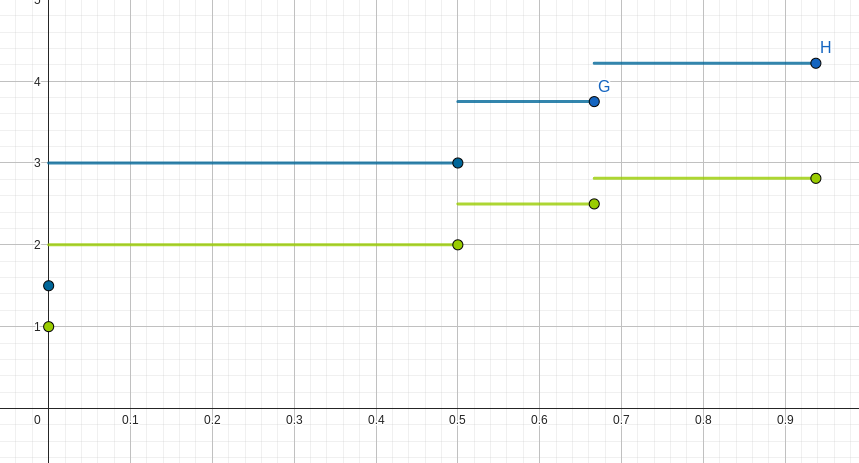
\includegraphics[width=1\linewidth]{fig2}
 	
 	
 	
 	
% \end{example} 




 \subsection{Operador de Poincaré} 
Llamaremos $\varphi_\alpha$ a solución  del problema de valores iniciales
 \begin{equation}
 	\left\lbrace \begin{array}{l}
 		d\varphi=f(t,\varphi(t))d\mu\\
 		\varphi(0)=\alpha,
 	\end{array}\right. \label{eq:Problema 0}
 \end{equation}
definida en \ref{def:sol}. De aquí  en adelante vamos a suponer que  $f:[0,T]\times\rr^n\to\rr^n$ está acotada, es decir $||f||_\infty<M$ y cumple con:
 \begin{enumerate}[label=\upshape(P-\arabic*),ref= (P-\arabic*)]
 	\item \label{pm1} Para cada $x\in\rr^n$, $f(t,x)$  $\mu$-medible en la variable $t$ y continua.
 	\item \label{pm2} Para cada $t\in[0,T]$, $f(t,x)$ es continua y acotada en la variable $x$.
 	\item \label{pm3} Existen $a,b$ positivos tal que
 	$$|f(t,x)|\leq a|x|+b.$$ 
 	\item \label{pm4}Existe $L\in\rr$ tal que $$\left| f(t,x)-f(t,y)\right|\leq L\left| x-y \right| . $$
 \end{enumerate} 
 Por el Teorema \ref{P-L}, para cada $\alpha$ existe una solución $\varphi_\alpha$ del problema de valores iniciales \eqref{eq:Problema 0}. Veamos qué propiedades tiene esta solución.
\begin{prop}
     Sea $\varphi_\alpha$ solución de  \eqref{eq:Problema 0}. Entonces $\varphi_{\alpha}\in L^\infty([0,T],\rr^n)$, y además si $s\leq t$, vale que
    \begin{equation*}\label{acotación}
        \left| \varphi_\alpha(t)-\varphi_\alpha(s)\right|\leq M\mu([s,t)).
    \end{equation*}
\end{prop}
\begin{proof}[Dem:]
 	Dado que $\varphi_{\alpha}$ es solución del problema \eqref{eq:Problema 0}, entonces por Definición  \ref{def:sol} tenemos que
 		$$\varphi_{\alpha}(t)=\varphi_{\alpha}(0)+\int_{[0,t)} f(s,\varphi_{\alpha}(s))\;d\mu,$$
 y por la desigualdad triangular vale que 
$$ 		|\varphi_{\alpha}(t)| \leq |\varphi_{\alpha}(0)|+\int_{[0,t)}| f(s,\varphi_{\alpha}(s))|\;d\mu.$$
Luego por \ref{pm3}
\begin{equation*}
\begin{split}
 	|\varphi_{\alpha}(t)| &\leq  |\varphi_{\alpha}(0)|+\int_{[0,t)}\left(a|\varphi_{\alpha}(s))|+b\right)\;d\mu\\	
     &\leq |\varphi_{\alpha}(0)|+b\mu([0,T])+a\int_{[0,t)}| \varphi_{\alpha}(s)|\;d\mu.
\end{split}
\end{equation*}
 Si llamamos $C=|\varphi_{\alpha}(0)|+b\mu([0,T])$ y $\nu=a\mu$, entonces
 $$|\varphi_{\alpha}(t)| \leq C+\int_{[0,t)}| \varphi_{\alpha}(s)|\;d\nu,$$
 aplicando el Teorema \ref{TG} obtenemos que para $t\in[0,T]$
 \begin{equation*}
 	|\varphi_{\alpha}(t)|\leq CK(T)\exp\left(K(T)a\bar{\mu}([0,T]) \right)  < \infty.
 \end{equation*}
Tomando supremo sobre todo el intervalo $[0,T]$, tenemos que\\
$\varphi_{\alpha}\in L^\infty([0,T],\rr^n).$
Por otro lado, como $||f||_\infty \leq M$, para $s\leq t$ vale que
  	\begin{equation*}
  		|\varphi_\alpha(t)-\varphi_\alpha(s)|\leq \int_{[s,t)}|f(r,\varphi_\alpha(r))|\;d\mu\leq M\;\mu\left( [s,t) \right). 
  	\end{equation*}
  
\end{proof}
\begin{cor}\label{corolario_continuidad}
    Sea $\varphi_\alpha$ solución de  \eqref{eq:Problema 0}. Si $t_0\in [0,T]$ cumple que $\mu(\{t_0\})=0$,  entonces $\varphi_\alpha$ es continua en $t_0$.
\end{cor}

\begin{proof}[Dem.]
Como $$0=\mu\left(\{t_0\}\right)=\mu\left(\bigcup_{n=1}^{\infty}\left[t_0-\frac{1}{n},t_0+\frac{1}{n}\right]\right)=\lim_{n\to\infty}\mu\left(\left[t_0-\frac{1}{n},t_0+\frac{1}{n}\right]\right)$$    
Para todo $\epsilon>0$ existe $N\in\nn$ tal que si $n>N$, entonces $$\mu\left(\left[t_0-\frac{1}{n},t_0+\frac{1}{n}\right]\right)<\epsilon/M.$$
Sea $\delta>0$ tal que  $\left[t_0-\delta,t_0+\delta\right]\subset\left[t_0-\frac{1}{n},t_0+\frac{1}{n}\right]$, entonces por la proposición \ref{acotación}, para $t\in \left[t_0-\delta,t_0+\delta\right]$ vale que
\begin{equation*}
    |\varphi_\alpha(t)-\varphi_\alpha(t_0)|\leq M\mu\left(\left[t_0-\frac{1}{n},t_0+\frac{1}{n}\right]\right)<\epsilon
\end{equation*}

\end{proof}




El siguiente teorema muestra que las soluciones de \eqref{eq:Problema 0}  están definidas en todo $[0,T]$.

 
 \begin{thm}[\textbf{Dominio de la solución}]\label{th:P(T)}
 	Sea $\mu$ una medida de Borel finita.   Si $f:[0,T]\times \rr^n\to\rr^n$  cumple con las condiciones \ref{pm1}  a \ref{pm4},  entonces la solución del problema \eqref{eq:Problema 0} está definida en todo el intervalo $[0,T]$.
 \end{thm}
 \begin{proof}[Dem.]
 	Supongamos que la solución máxima está definida en el intervalo $[0,t_1]$, donde $t_1< T$. Entonces por el Teorema  \ref{th:extensión} se debe cumplir alguna de las dos condiciones:
 	\begin{enumerate}
 		\item[A)] 	$\forall K\Subset [0,T)\times\rr^n$ existe $t_2\in [0,t_1)$ tal que $(t,\varphi(t))\notin K$   $\forall t\in(t_2,t_1)$. 

        \item[B)] Existe $x_1=\lim\limits_{t\to t_1^-}\varphi(t)$,  $(t_1,x_1)\in[0,T)\times\rr^n$ y  $$\left( t_1 , \varphi(t_1)+f(t_1,\varphi(t_1))\mu(\{t_1\})\right) \notin [0,T)\times\rr^n.$$
\end{enumerate}


   
 Si la condición (A) es verdadera, entonces para
 		$\epsilon\in\left( 0,\dfrac{T-t_1}{2}\right)$ 
    definimos el conjunto $K_{\epsilon}=[0,t_1+\epsilon]\times B(0,R)$ donde $||\varphi||_\infty\leq R$. Como $K_{\epsilon}$ es cerrado y acotado, entonces $K_{\epsilon}$ está compactamente incluido en $[0,T)\times\rr^n$. Luego existe $t_2\in [0,t_1)$ tal que $(t,\varphi(t))\notin K_{\epsilon}$ para todo $t\in(t_2,t_1)$.  Como $\varphi(t)\in B(0,R)$, la única manera de que  $(t,\varphi(t))\notin K_{\epsilon}$ es que  $t>t_1+\epsilon$, lo cual es un absurdo. Por otro lado, es inmediato que  (B) es falso,  porque si no lo fuese, resultaría que $\varphi(t_1)+f(t_1,\varphi(t_1))\mu(\{t_1\})\notin\rr^n$. Luego el intervalo donde está definida $\varphi$ es $[0,T]$.
 \end{proof}


\begin{defi} \label{def:op-poincare}
 Llamaremos operador de Poincaré  al operador $P:\rr^n\to \rr^n$ tal que para cada valor inicial $\alpha$,\index{operador de Poincaré} $P(\alpha)=\varphi_\alpha(T)$, \index[Simbolo]{$P$} donde $\varphi_\alpha$ es solución de \eqref{eq:Problema 0}.
\end{defi}

 
 \begin{lem}
    El operador de Poincaré es continuo.\label{opr continuo}
\end{lem}
\begin{proof}[Dem.]
 Sean $\varphi_\alpha$ y $\varphi_\beta$ dos soluciones del problema \eqref{eq:Problema 0}. Como $f$ es Lipschitz 
 \begin{equation*}
 \begin{split}
 	| \varphi_\alpha(t)-\varphi_\beta(t)|&\leq |\alpha-\beta |+\int_{[0,t)} |f(r,\varphi_\alpha(r)) -f(t,\varphi_\beta(t))| \; d|\mu|\\
	&\leq |\alpha-\beta|+L\int_{[0,t)} |\varphi_\alpha(r) -\varphi_\beta(t)| \; d|\mu|.
 \end{split}
\end{equation*}
 Si aplicamos el Teorema \ref{TG} tomando $u(t)=|\varphi_\alpha(t)-\varphi_\beta(t)|$, $c=|\alpha-\beta|$ y  $\nu=L|\mu|$, conseguimos

\begin{equation*}
|\varphi_\alpha(t)-\varphi_\beta(t)|\leq K(t) |\alpha-\beta|e^{K(t)L\bar{|\mu|}([t_0,t))}.
\end{equation*}
Luego, si evaluamos en $t=T$ y llamamos  $K=K(T)=\displaystyle\prod_{\tau\in D}\mu(\{\tau\})<\infty$.
 

\begin{equation*}
 		|P(\alpha)-P(\beta)|=|\varphi_{\alpha}(T)-\varphi_{\beta}(T)|_{1}\leq K |\alpha-\beta|_{1}e^{KL\bar{|\mu|}([0,T))}\to 0
 	\end{equation*}
 cuando $|\alpha-\beta|\to 0$.
\end{proof}
 
 
 

%\begin{obs} \label{ob: cont P}
 %	Por \ref{th:P(T)}  el operador de Poincaré está bien definido, ya que la solución se puede extender a todo el intervalo $[0,T]$. Además por \ref{opr continuo} el operador es continuo.
 %\end{obs} 
 
 

 \begin{thm} \label{th: P}
 	Sea $R>0$ y $f$ satisface las condiciones \ref{pm1} a \ref{pm4}, \ref{fun-tele} para $B(0,R)$  y  además que
 	\begin{equation}
 		f(t,u)\cdot u<0 \text{ para todo par } (t,u) \text{ donde }  |u| =R  \text{ y   } \mu(\{t\})=0.  \label{eq:4}
 	\end{equation}
 Entonces el operador de Poincaré definido en \ref{def:op-poincare} cumple que \\
 $P\left(  \overline{B(0,R)}\right)  \subset \overline{B(0,R)}$.
 \end{thm}
 
 \begin{proof}[Dem.] Sea $\varphi_\alpha$  la solución a \ref{eq:Problema 0} y sea $A=\{t\in [0,T] \mid \varphi_\alpha(s)\in \overline{B(0,R)}, \; \forall s\in [0,t]\}$, veamos que el conjunto $A$ es simultáneamente abierto y cerrado relativo al intervalo $[0,T]$, y  como $[0,T]$ es conexo, entonces $A=[0,T]$.
  
 Veamos primero que  $A$  es un conjunto cerrado respecto al $[0,T]$. Para ello, sea   $t_n$  una sucesión de $A$ que converge a $t$, veamos que $t\in A$.  Si para algún $n$, $t_n\geq t$ entonces $\forall s \in [0,t]\subset [0,t_n] $ vale que $\varphi_\alpha(s)\in\overline{B(0,R)}$,  por lo tanto en $t\in A$.  Si por el contrario $\forall n$ tenemos que $t_n < t$,  como $\varphi_\alpha$ es continua a izquierda, entonces $\lim\limits_{n\to \infty}\varphi_\alpha(t_n)=\varphi_\alpha(t)$ y como cada $\varphi_\alpha(t_n)\in \overline{B(0,R)}$ es inmediato que $\varphi_\alpha(t)\in \overline{B(0,R)}$, es decir $t\in A$.  Por lo tanto, $A$ es cerrado.
 	 
  	Si $A$ es un conjunto abierto relativo al $[0,T]$, entonces $[0,T]\setminus A$ es cerrado, es decir para toda sucesión $\{t_n\}\subset [0,T]\setminus A$ si $t_n\to t$ entonces $t\in[0,T]\setminus A$. Por lo tanto si suponemos que  $A$ no es abierto relativo al intervalo $[0,T]$, entonces $\exists t_0\in A$ y $\{t_n\}\nsubset A$ tal que $t_n\to t_0$. Podemos asegurar que si $t> t_0$ entonces $t\notin A$, pues existe $n_0$ tal que $t_0<t_{n_0}<t$ y como tengo que $t_{n_0}\notin A$, en particular $|\varphi_\alpha(t_{n_0})|>R$.
   
   Veamos que como $t_0\in A$, entonces $\varphi_\alpha(t_0)\in B(0,R)$ o  $\varphi_\alpha(t_0)\in \partial B(0,R) $, y siempre existe $t> t_0$ tal que $t\in A$.%$|\varphi(t)|\in \overline{B(0,R)}$.% 
 		\begin{itemize}
   		\item Supongamos que $\varphi_\alpha(t_0)\in B(0,R)$.
     \end{itemize}
En el problema \eqref{eq:Problema 0} podemos tomar como condición inicial $\varphi(0)=\varphi_\alpha(t_0)=\beta\in B(0,R)$, entonces por el Teorema \ref{P-L} existe una solución, que notaremos  $\varphi_{\beta}$. Luego, tenemos que para todo $t\in [0,\delta)$ el par $(t,\varphi_\beta(t))\in \Omega$, donde  $\Omega$ es un entorno de $[0,T]\times B(0,R)$. Ahora podemos extender a $\varphi_\alpha $ de la siguiente manera
$$\varphi_\alpha(t)=\left\{\begin{array}{ccc}
    \varphi_\alpha(t) & si &  t\in[0,t_0)\\
     \varphi_\beta(t-t_0) & si &t\in[t_0,t_0+\delta) 
\end{array}\right.$$
Por lo tanto para todo $t\in[t_0,t_0+\delta)$ vale que $|\varphi_\alpha(t)|=|\varphi_\beta(t-t_0)|\leq R$. Es decir existe $t>t_0$ tal que $t\in A$.

    
    \begin{itemize}
        
    
    \item Supongamos que  $\varphi(t_0)\in \partial B(0,R)$ y $\mu(\{t_0\})\neq 0$.
    
    \end{itemize}
Por \eqref{fun-tele}  $x_1=\varphi(t_0)+f(t,\varphi(t_0))\mu(\{t_0\})\in B(0,R)$, y tomando la medida $\hat{\mu}=\mu-\mu(\{t_0\})\delta_{t_0}$, es claro que $\hat{\mu}(\{t_0\})=0$, puedo aplicar el Teorema \ref{P-L} para la condición inicial $\varphi(0)=x_1$, pero con la medida $\hat{\mu}$.  Luego, existe $\delta>0$  y $\varphi_{x_1}$ tal que $|\varphi_{x_1}(t)|\leq R$ para todo $t\in [0,0+\delta)$. Ahora puedo extender la solución $\varphi_\alpha$ al intervalo $[0,t_0+\delta)$  de la siguiente manera
$$\varphi_\alpha(t)=\left\{\begin{array}{ccc}
    \varphi_\alpha(t) & si &  t\in[0,t_0]\\
     \varphi_{x_1}(t-t_0) & si &t\in(t_0,t_0+\delta) 
\end{array}\right.$$
Por lo tanto existe $t>t_0$ tal que $|\varphi_\alpha(t)|<R$, es decir vale que $t\in A$.



% \begin{multline*}
 %	|\hat{\mu}|\left( \{t_0\}\right) =|\hat{\mu}|\left( \bigcap_{n=1}^\infty[t_0,t_0+1/n)\right)=\lim\limits_{n\to\infty}|\hat{\mu}|\left( [t_0,t_0+1/n) \right) =0
 %\end{multline*} 
 %existe $N>0$ que $|\hat{\mu}\left( [t_0,t_0+1/N]\right)\leq R/M $. Por lo tanto puedo aplicar el Teorema de Existencia y Unicidad para las condiciones $(t_0,x_1)$ y la medida $\hat{\mu}$, por el cual va a  existir $\delta$ tal que el problema \refeq{Problema P} tiene solución en el intervalo $[t_0,t_0+\delta]$,  es decir podemos extender la solución del problema hasta el intervalo $[0,t_0+\delta]$ lo cual contradice que $A$ no sea abierto.
 		



    
\begin{itemize}
\item Supongamos $\varphi(t_0)\in \partial B(0,R)$ y $\mu(\{t_0\})= 0$ 
\end{itemize}
De \eqref{eq:4} existe $b>0$ tal que $f(t_0,\varphi(t_0))\cdot\varphi(t_0)<-b$.

Por \eqref{f lipschitz} y Corolario \ref{corolario_continuidad}, para $\epsilon=\frac{b}{3RL}$ existe $\delta_1>0$ tal que si $t\in[t_0,t_0+\delta_1)$ entonces
\begin{equation}
    \begin{split}
        \int_{[t_0,t)} f(s,\varphi_\alpha(s))-f(s,\varphi_\alpha(t_0))\; d\mu& \leq \int_{[t_0,t)} |\varphi_\alpha(s)\varphi_\alpha(t_0)|\; d\mu \\ &\leq \frac{b}{3R}\mu((t_0,t)).
    \end{split}\label{eq:A}
\end{equation}
Además, como $f$ es continua en $t_0$ $\exists \delta_2>0 $ tal que si $s\in [t_0,t_0+\delta_2)$, entonces
\begin{equation}
    |f(s,\varphi_\alpha(t_0))-f(t_0,\varphi_\alpha(t_0))|\leq \frac{b}{3R}.\label{eq:B}
\end{equation}

Para todo $t\in[t_0,t_0+\delta)$, donde $\delta=\min\{\delta_1,\delta_2\}$, usando \eqref{eq:A} y \eqref{eq:B} tenemos que 
\begin{equation*}
    \begin{split}
    \varphi_\alpha(t)-\varphi_\alpha(t_0) &= \int_{(t_0,t)}\left[f(s,\varphi_\alpha(s))-f(s,\varphi_\alpha(t_0))\right]\; d\mu\\& + \int_{(t_0,t)}\left[f(s,\varphi_\alpha(t_0))-f(t_0,\varphi_\alpha(t_0))\right]\; d\mu \\&+ \int_{(t_0,t)}f(t_0,\varphi_\alpha(t_0))\; d\mu,\\
& \leq \frac{b}{3R}\mu((t_0,t)) + \int_{(t_0,t)}\frac{b}{3R}\; d\mu + \int_{(t_0,t)}f(t_0,\varphi_\alpha(t_0))\; d\mu.
\end{split}
\end{equation*}		 
Si multiplicamos por el vector $\varphi_\alpha(t_0)$ y como $|\varphi_\alpha(t_0)|=R$, entonces
\begin{equation*}
\begin{split}
\left[\varphi_\alpha(t)-\varphi_\alpha(t_0)\right]\cdot \varphi_\alpha(t_0) \leq & \varphi_\alpha(t_0)\frac{2b}{3R}\mu((t_0,t))\\& + \int_{(t_0,t)}f(t_0,\varphi_\alpha(t_0))\cdot \varphi_\alpha(t_0)\; d\mu\\
&\leq \frac{2b}{3}\mu((t_0,t))-b\mu((t_0,t))=-\frac{b}{3}\mu((t_0,t)).
\end{split}
\end{equation*}
Luego por la Proposición?? \eqref{acotación}
\begin{equation*}
    \begin{split}
    |\varphi_\alpha(t)|^2=&|\varphi_\alpha(t_0)|^2+2\left[\varphi_\alpha(t)-\varphi_\alpha(t_0)\right]\cdot\varphi_\alpha(t_0)+|\varphi_\alpha(t)-\varphi_\alpha(t_0)|^2\\
   &\leq R^2-\dfrac{2b}{3}\mu((t_0,t))+M^2 \mu((t_0,t))^2.  
    \end{split}
\end{equation*}
O equivalentemente
\begin{equation}
    |\varphi_\alpha(t)|^2-R^2\leq \mu((t_0,t))\left[M^2 \mu((t_0,t))-\dfrac{2b}{3}\right]. 
\end{equation}
El término de la derecha es una expresión cuadrática respecto a $\mu((t_0,t))$, y tiene como raíces $t_0$ y  otro valor a derecha de $t_0$, es decir existe $t_1>t_0$ tal que $|\varphi_\alpha(t_1)|^2-R^2\leq 0$, por lo tanto $t_1\in A$.
  		
Por lo tanto, mostramos que existe $t_1>t_0$ tal que $t\in A$, lo cual contradice que no sea abierto relativo al $[0,T]$. Finalmente, si $A$ es abierto y cerrado relativo al intervalo $[0,T]$, entonces $A=[0,T]$.
 	
Luego, para cualquier $\alpha\in\overline{B(0,R)}$, $$P(\alpha)=\varphi_\alpha(T)\in\overline{B(0,R)}.$$ 
 \end{proof}
 
 \begin{thm}[\textbf{Teorema de Brouwer}]
 	
 	Sea $B(0,R)$ una bola de $\rr^n$  y sea $P:\overline{B(0,R)}\to \overline{B(0,R)}$ continua. Entonces existe $x \in \overline{B(0,R)}$ tal que $P(x) = x$.
 \end{thm}
 \begin{thm} \label{th:final}
 	Sea $\mu$ una medida de Borel finita, y sea $f:[0,T]\times\rr^n\to\rr^n$ una función que cumple con las condiciones \ref{pm1} a \ref{pm4}. Además, existe una bola $B(0,R)$ tal que si $x\in\overline{B(0,R)}$, entonces
    $x+f(t,x)\mu(\{t\})\in \overline{B(0,R)}$ para todo $t\in[0,T]$, y
 	$$f(t,x)\cdot x<0 \; \text{ para todos}\; |x|=R \;\text{y}\; \mu(\{t\})=0.$$
 	Entonces el problema
 	 \begin{equation}
 		\left\lbrace \begin{array}{l}
 			d(\varphi)=f(t,\varphi(t))d\mu\\
 			\varphi(0)=\varphi(T)
 		\end{array}\right. \tag{${PP}$}
 	\end{equation} 
tiene al menos una solución. 
\end{thm}
 \begin{proof}[Dem.]
 	Por el Teorema \ref{th:P(T)} y el Lema  \ref{opr continuo}, el operador $P$ está bien definido y es continuo. Luego, por el Teorema  \ref{th: P} se tiene que $P\left( \overline{B(0,R)}\right)\subset\overline{B(0,R)} $, y ahora aplicando el Teorema de Brouwer  se llega a que existe una solución $\varphi$ al problema \eqref{eq:Problema 0} tal que $\varphi(T)=\varphi(0).$
 \end{proof}

 \begin{example}\label{ejemplo vectorial}
 	Sea $u:[0,T]\to \rr$, y sean $g_{1,2}:[0,T]\to \rr^n$  funciones suficientemente buenas, definimos el siguiente problema impulsivo
 	 \begin{equation}\label{eq:ejemplo 3}
 		\left\lbrace \begin{array}{l}
    u''=g_1(t,u,u')d\lambda+g_2(t,u,u') \displaystyle\sum_{i=1}^rd\delta_{t_i}\\
 			u'(0)=u'(T)\\
 			u(0)=u(T),
 		\end{array}\right. 
 	\end{equation} 
 donde $t_i\in(0,T)$ y $\delta_{t_i}$ es la medida delta de Dirac concentrada en $t_i$. Veamos como podemos aplicar el teorema \ref{th:final} a este tipo de problemas.
 
 Si llamamos $u'=v$  podemos transformar el problema \eqref{eq:ejemplo 3} en un sistema de ecuaciones
  \begin{equation*}
 	\left\lbrace \begin{array}{l}
 		(u',v')=\left(v, g_1(t,u,v)\right)d\lambda +\displaystyle\sum_{i=1}^r\left(0,g_2(t,u,v)\right)d \delta_{t_i}\\
   (u(0),v(0))=(u(T),v(T)).
 	\end{array}\right. 
 \end{equation*} 
A este sistema de ecuaciones lo podemos escribir de manera vectorial, tomando $\varphi=(u,v)$, $G_1(t,\varphi)=(v,g(t,u,v))$ y $G_2(t,\varphi)=(0,g_2(t,u,v))$.
  \begin{equation*}
	\left\lbrace \begin{array}{l}
	\varphi'=G_1(t,\varphi)d\lambda+G_2(t,\varphi)\displaystyle\sum_{i=1}^r d \delta_{t_i}\\
 \varphi(0)=\varphi(T).
	\end{array}\right. 
\end{equation*} 
Si llamamos $F(t,\varphi)=\left( G_1(t,\varphi)\chi_{[0,T]-\{t_1,..,t_r\}}+G_2(t,\varphi)\chi_{\{t_1,...,t_r\}}\right) $ y tomando $d\mu=d\left(\lambda+\displaystyle\sum_{i=1}^r\delta_{t_i}\right)$, entonces la ecuación vectorial se transforma en la del Teorema \ref{th:final}. 
 \end{example}